% Options for packages loaded elsewhere
\PassOptionsToPackage{unicode}{hyperref}
\PassOptionsToPackage{hyphens}{url}
\PassOptionsToPackage{dvipsnames,svgnames*,x11names*}{xcolor}
%
\documentclass[
  12pt, krantz2,
]{krantz}
\usepackage{lmodern}
\usepackage{amssymb,amsmath}
\usepackage{ifxetex,ifluatex}
\ifnum 0\ifxetex 1\fi\ifluatex 1\fi=0 % if pdftex
  \usepackage[T1]{fontenc}
  \usepackage[utf8]{inputenc}
  \usepackage{textcomp} % provide euro and other symbols
\else % if luatex or xetex
  \usepackage{unicode-math}
  \defaultfontfeatures{Scale=MatchLowercase}
  \defaultfontfeatures[\rmfamily]{Ligatures=TeX,Scale=1}
  \setmonofont[Scale=0.7]{Source Code Pro}
\fi
% Use upquote if available, for straight quotes in verbatim environments
\IfFileExists{upquote.sty}{\usepackage{upquote}}{}
\IfFileExists{microtype.sty}{% use microtype if available
  \usepackage[]{microtype}
  \UseMicrotypeSet[protrusion]{basicmath} % disable protrusion for tt fonts
}{}
\makeatletter
\@ifundefined{KOMAClassName}{% if non-KOMA class
  \IfFileExists{parskip.sty}{%
    \usepackage{parskip}
  }{% else
    \setlength{\parindent}{0pt}
    \setlength{\parskip}{6pt plus 2pt minus 1pt}}
}{% if KOMA class
  \KOMAoptions{parskip=half}}
\makeatother
\usepackage{xcolor}
\IfFileExists{xurl.sty}{\usepackage{xurl}}{} % add URL line breaks if available
\IfFileExists{bookmark.sty}{\usepackage{bookmark}}{\usepackage{hyperref}}
\hypersetup{
  pdftitle={HR Analytics in R},
  pdfauthor={Chester Ismay, Albert Y. Kim and Hendrik Feddersen},
  colorlinks=true,
  linkcolor=Maroon,
  filecolor=Maroon,
  citecolor=Blue,
  urlcolor=Blue,
  pdfcreator={LaTeX via pandoc}}
\urlstyle{same} % disable monospaced font for URLs
\usepackage{color}
\usepackage{fancyvrb}
\newcommand{\VerbBar}{|}
\newcommand{\VERB}{\Verb[commandchars=\\\{\}]}
\DefineVerbatimEnvironment{Highlighting}{Verbatim}{commandchars=\\\{\}}
% Add ',fontsize=\small' for more characters per line
\usepackage{framed}
\definecolor{shadecolor}{RGB}{248,248,248}
\newenvironment{Shaded}{\begin{snugshade}}{\end{snugshade}}
\newcommand{\AlertTok}[1]{\textcolor[rgb]{0.33,0.33,0.33}{#1}}
\newcommand{\AnnotationTok}[1]{\textcolor[rgb]{0.37,0.37,0.37}{\textbf{\textit{#1}}}}
\newcommand{\AttributeTok}[1]{\textcolor[rgb]{0.61,0.61,0.61}{#1}}
\newcommand{\BaseNTok}[1]{\textcolor[rgb]{0.06,0.06,0.06}{#1}}
\newcommand{\BuiltInTok}[1]{#1}
\newcommand{\CharTok}[1]{\textcolor[rgb]{0.5,0.5,0.5}{#1}}
\newcommand{\CommentTok}[1]{\textcolor[rgb]{0.37,0.37,0.37}{\textit{#1}}}
\newcommand{\CommentVarTok}[1]{\textcolor[rgb]{0.37,0.37,0.37}{\textbf{\textit{#1}}}}
\newcommand{\ConstantTok}[1]{\textcolor[rgb]{0,0,0}{#1}}
\newcommand{\ControlFlowTok}[1]{\textcolor[rgb]{0.27,0.27,0.27}{\textbf{#1}}}
\newcommand{\DataTypeTok}[1]{\textcolor[rgb]{0.27,0.27,0.27}{#1}}
\newcommand{\DecValTok}[1]{\textcolor[rgb]{0.06,0.06,0.06}{#1}}
\newcommand{\DocumentationTok}[1]{\textcolor[rgb]{0.37,0.37,0.37}{\textbf{\textit{#1}}}}
\newcommand{\ErrorTok}[1]{\textcolor[rgb]{0.14,0.14,0.14}{\textbf{#1}}}
\newcommand{\ExtensionTok}[1]{#1}
\newcommand{\FloatTok}[1]{\textcolor[rgb]{0.06,0.06,0.06}{#1}}
\newcommand{\FunctionTok}[1]{\textcolor[rgb]{0,0,0}{#1}}
\newcommand{\ImportTok}[1]{#1}
\newcommand{\InformationTok}[1]{\textcolor[rgb]{0.37,0.37,0.37}{\textbf{\textit{#1}}}}
\newcommand{\KeywordTok}[1]{\textcolor[rgb]{0.27,0.27,0.27}{\textbf{#1}}}
\newcommand{\NormalTok}[1]{#1}
\newcommand{\OperatorTok}[1]{\textcolor[rgb]{0.43,0.43,0.43}{\textbf{#1}}}
\newcommand{\OtherTok}[1]{\textcolor[rgb]{0.37,0.37,0.37}{#1}}
\newcommand{\PreprocessorTok}[1]{\textcolor[rgb]{0.37,0.37,0.37}{\textit{#1}}}
\newcommand{\RegionMarkerTok}[1]{#1}
\newcommand{\SpecialCharTok}[1]{\textcolor[rgb]{0,0,0}{#1}}
\newcommand{\SpecialStringTok}[1]{\textcolor[rgb]{0.5,0.5,0.5}{#1}}
\newcommand{\StringTok}[1]{\textcolor[rgb]{0.5,0.5,0.5}{#1}}
\newcommand{\VariableTok}[1]{\textcolor[rgb]{0,0,0}{#1}}
\newcommand{\VerbatimStringTok}[1]{\textcolor[rgb]{0.5,0.5,0.5}{#1}}
\newcommand{\WarningTok}[1]{\textcolor[rgb]{0.37,0.37,0.37}{\textbf{\textit{#1}}}}
\usepackage{longtable,booktabs}
% Correct order of tables after \paragraph or \subparagraph
\usepackage{etoolbox}
\makeatletter
\patchcmd\longtable{\par}{\if@noskipsec\mbox{}\fi\par}{}{}
\makeatother
% Allow footnotes in longtable head/foot
\IfFileExists{footnotehyper.sty}{\usepackage{footnotehyper}}{\usepackage{footnote}}
\makesavenoteenv{longtable}
\usepackage{graphicx,grffile}
\makeatletter
\def\maxwidth{\ifdim\Gin@nat@width>\linewidth\linewidth\else\Gin@nat@width\fi}
\def\maxheight{\ifdim\Gin@nat@height>\textheight\textheight\else\Gin@nat@height\fi}
\makeatother
% Scale images if necessary, so that they will not overflow the page
% margins by default, and it is still possible to overwrite the defaults
% using explicit options in \includegraphics[width, height, ...]{}
\setkeys{Gin}{width=\maxwidth,height=\maxheight,keepaspectratio}
% Set default figure placement to htbp
\makeatletter
\def\fps@figure{htbp}
\makeatother
\setlength{\emergencystretch}{3em} % prevent overfull lines
\providecommand{\tightlist}{%
  \setlength{\itemsep}{0pt}\setlength{\parskip}{0pt}}
\setcounter{secnumdepth}{5}
\usepackage{booktabs}
\usepackage{longtable}
\usepackage[bf,singlelinecheck=off]{caption}

\usepackage{framed,color}
\definecolor{shadecolor}{RGB}{248,248,248}

\usepackage{float}
\usepackage{array}
\usepackage{multirow}
%\usepackage[table]{xcolor}
\usepackage{wrapfig}
\usepackage{colortbl}
\usepackage{pdflscape}
\usepackage{tabu}
\usepackage{threeparttable}
\usepackage{threeparttablex}
\usepackage[normalem]{ulem}
\usepackage{makecell}

\renewcommand{\textfraction}{0.05}
\renewcommand{\topfraction}{0.8}
\renewcommand{\bottomfraction}{0.8}
\renewcommand{\floatpagefraction}{0.75}

\renewenvironment{quote}{\begin{VF}}{\end{VF}}
\let\oldhref\href
\renewcommand{\href}[2]{#2\footnote{\url{#1}}}

\makeatletter
\newenvironment{kframe}{%
\medskip{}
\setlength{\fboxsep}{.8em}
 \def\at@end@of@kframe{}%
 \ifinner\ifhmode%
  \def\at@end@of@kframe{\end{minipage}}%
  \begin{minipage}{\columnwidth}%
 \fi\fi%
 \def\FrameCommand##1{\hskip\@totalleftmargin \hskip-\fboxsep
 \colorbox{shadecolor}{##1}\hskip-\fboxsep
     % There is no \\@totalrightmargin, so:
     \hskip-\linewidth \hskip-\@totalleftmargin \hskip\columnwidth}%
 \MakeFramed {\advance\hsize-\width
   \@totalleftmargin\z@ \linewidth\hsize
   \@setminipage}}%
 {\par\unskip\endMakeFramed%
 \at@end@of@kframe}
\makeatother

\renewenvironment{Shaded}{\begin{kframe}}{\end{kframe}}

\usepackage{makeidx}
\makeindex

\urlstyle{tt}

%% Need to clean up
\newenvironment{rmdblock}[1]
  {\begin{shaded*}
  \begin{itemize}
  \renewcommand{\labelitemi}{
    \raisebox{-.7\height}[0pt][0pt]{
  %    {\setkeys{Gin}{width=3em,keepaspectratio}\includegraphics{images/#1}}
    }
  }
  \item
  }
  {
  \end{itemize}
  \end{shaded*}
  }

\newenvironment{rmdnote}
  {\begin{rmdblock}{note}}
  {\end{rmdblock}}
\newenvironment{rmdcaution}
  {\begin{rmdblock}{caution}}
  {\end{rmdblock}}
\newenvironment{rmdimportant}
  {\begin{rmdblock}{important}}
  {\end{rmdblock}}
\newenvironment{rmdtip}
  {\begin{rmdblock}{tip}}
  {\end{rmdblock}}
\newenvironment{rmdwarning}
  {\begin{rmdblock}{warning}}
  {\end{rmdblock}}
\newenvironment{learncheck}
  {\begin{rmdblock}{warning}}
  {\end{rmdblock}}
\newenvironment{review}
  {\begin{rmdblock}{warning}}
  {\end{rmdblock}}
\newenvironment{announcement}
  {\begin{rmdblock}{warning}}
  {\end{rmdblock}}


\usepackage{amsthm}
\makeatletter
\def\thm@space@setup{%
  \thm@preskip=8pt plus 2pt minus 4pt
  \thm@postskip=\thm@preskip
}
\makeatother

\frontmatter
\usepackage[]{natbib}
\bibliographystyle{apalike}

\title{HR Analytics in R}
\usepackage{etoolbox}
\makeatletter
\providecommand{\subtitle}[1]{% add subtitle to \maketitle
  \apptocmd{\@title}{\par {\large #1 \par}}{}{}
}
\makeatother
\subtitle{Common tasks achieved with the power of R}
\author{Chester Ismay, Albert Y. Kim and Hendrik Feddersen}
\date{May 11, 2019}

\begin{document}
\maketitle

% you may need to leave a few empty pages before the dedication page

%\cleardoublepage\newpage\thispagestyle{empty}\null
%\cleardoublepage\newpage\thispagestyle{empty}\null
%\cleardoublepage\newpage
\thispagestyle{empty}

\begin{center}
%\includegraphics{images/dedication.pdf}
\end{center}

\setlength{\abovedisplayskip}{-5pt}
\setlength{\abovedisplayshortskip}{-5pt}

{
\hypersetup{linkcolor=}
\setcounter{tocdepth}{2}
\tableofcontents
}
\listoftables
\listoffigures
\mainmatter

\hypertarget{intro}{%
\chapter{Introduction}\label{intro}}

\begin{center}\rule{0.5\linewidth}{\linethickness}\end{center}

\begin{learncheck}
\textbf{Please note that you are currently looking at the latest version
of ``HR Analytics in R''. However, since work is still in progress it is
subject to frequent change.}
\end{learncheck}

The intention of this book is to encourage more `data driven' decisions in HR. HR Analytics is not anymore a nice-to-have addon but rather the way HR practitioners should conduct HR decision making in the future. Where applicable, human judgement is `added' onto a rigorous analysis of the data done in the first place.

To achieve this ideal world, I need to equip you with some fundamental knowledge of R and RStudio, which are open-source tools for data scientists. I am well aware that on one side you want to do something for your career in HR, however you are most likely completely new to coding.

\textbf{Help! I'm new to R and RStudio. I'm completely new to coding! What shall I do?}


\includegraphics[width=\textwidth,height=0.2\textheight]{images/Rlogo.png} \hfill         
\includegraphics[width=\textwidth,height=0.2\textheight]{images/RStudio-Logo-Blue-Gradient.png}

If you're asking yourself this question, then you have come to the right place! There is no better moment to ride the wave of disruptions taking place now in HR.

\begin{itemize}
\tightlist
\item
  \emph{Are you looking to learn about HR Analytics utilising the power of R"? Then start with our \protect\hyperlink{sec:intro-for-students}{Introduction for Students}.}
\item
  \emph{Are you looking to contribute to ``HR Analytics in R''? Then click \protect\hyperlink{sec:connect-contribute}{here} for information on how.}
\item
  \emph{Are you curious about the publishing of this book? Then click \protect\hyperlink{sec:about-book}{here} for more information on the open-source technology, in particular R Markdown and the bookdown package.}
\end{itemize}

This is version 0.5.0 of ``HR Analytics in R'' published on May 11, 2019. While a PDF version of this book can be found \href{hendrikfeddersen.pdf}{here}, this is very much a work in progress with many things that still need to be fixed. I appreciate your patience.

\begin{center}\rule{0.5\linewidth}{\linethickness}\end{center}

\hypertarget{sec:intro-for-students}{%
\section{Introduction for students}\label{sec:intro-for-students}}

This book assumes no prerequisites: no algebra, no calculus, and no prior programming/coding experience. This is intended to be a gentle introduction to the practice of analyzing data and answering questions using data the way data scientists, statisticians and other researchers would.

\hypertarget{workingwithmaterials}{%
\subsection*{Working with the material}\label{workingwithmaterials}}


You can work your way through the materials by clicking on the arrows to the left and right at the bottom of each page. Alternatively, there is a collapsible contents bar on the left hand side.

If you need to find something specific, you can use the search icon. Typing in a word or phrase will filter the contents bar to relevant sections.

The book by default renders black sans serif on a white background. You can use the A to amend the appearance of the book to make it easier to process, whether that's a larger font, a serif font, or a different colour scheme.

The edit button takes you straight to github, where you can propose editorial changes.

\hypertarget{conventions}{%
\subsection*{Conventions}\label{conventions}}


Throughout this book various conventions will be used.

In terms of basic formatting:

\begin{itemize}
\tightlist
\item
  This is standard text.
\item
  \texttt{This\ is\ code\ or\ a\ symbol}
\item
  \emph{This is a Keyboard Key!}
\item
  \textbf{This is the first time I mention something important}
\end{itemize}

This is a book about coding, so expect code blocks. Code blocks will typically look like this:

\begin{Shaded}
\begin{Highlighting}[]
\StringTok{"this is a code block"}
\end{Highlighting}
\end{Shaded}

\begin{verbatim}
[1] "this is a code block"
\end{verbatim}

Directly underneath it, normally starting with two hash symbols (\#\#) is the result of the code executing.

\begin{Shaded}
\begin{Highlighting}[]
\CommentTok{## [1] 'this is a code block'`}
\end{Highlighting}
\end{Shaded}

There will also be callouts throughout the book. Some are for information, some expect you to do things.

Anything written here should be read carefully before proceeding.

This is a tip relating to what I've just said.

This is kind of like a tip but is for when you're getting into trouble and need help.

This is something I recommend you do as you're reading.

In Figure \ref{fig:moderndive-figure} I present a flowchart of what you'll cover in this book. You'll first get started with data in Chapter \ref{getting-started}, where you'll learn about the difference between R and RStudio, start coding in R, understand what R packages are, and explore your first dataset: all domestic departure flights from a New York City airport in 2013. Then

\begin{enumerate}
\def\labelenumi{\arabic{enumi}.}
\tightlist
\item
  \textbf{Data science}: You'll assemble your data science toolbox using \texttt{tidyverse} packages. In particular:

  \begin{itemize}
  \tightlist
  \item
    Ch.\ref{viz}: Visualizing data via the \texttt{ggplot2} package.
  \item
    Ch.\ref{tidy}: Understanding the concept of ``tidy'' data as a standardized data input format for all packages in the \texttt{tidyverse}
  \item
    Ch.\ref{wrangling}: Wrangling data via the \texttt{dplyr} package.
  \end{itemize}
\item
  \textbf{Data modeling}: Using these data science tools and helper functions from the \texttt{moderndive} package, you'll start performing data modeling. In particular:

  \begin{itemize}
  \tightlist
  \item
    Ch.\ref{regression}: Constructing basic regression models.
  \item
    Ch.\ref{multiple-regression}: Constructing multiple regression models.
  \end{itemize}
\item
  \textbf{Statistical inference}: Once again using your newly acquired data science tools, I'll unpack statistical inference using the \texttt{infer} package. In particular:

  \begin{itemize}
  \tightlist
  \item
    Ch.\ref{sampling}: Understanding the role that sampling variability plays in statistical inference using both tactile and virtual simulations of sampling from a ``bowl'' with an unknown proportion of red balls.
  \item
    Ch.\ref{confidence-intervals}: Building confidence intervals.
  \item
    Ch.\ref{hypothesis-testing}: Conducting hypothesis tests.
  \end{itemize}
\item
  \textbf{Data modeling revisited}: Armed with your new understanding of statistical inference, you'll revisit and review the models you constructed in Ch.\ref{regression} \& Ch.\ref{multiple-regression}. In particular:

  \begin{itemize}
  \tightlist
  \item
    Ch.\ref{inference-for-regression}: Interpreting both the statistical and practice significance of the results of the models.
  \item
    Ch.\ref{thinking-with-data}: I'll end the introductory chapters with a discussion on what it means to ``think with data'' and present an example case study data analysis of house prices in Seattle.
  \end{itemize}
\item
  \textbf{HR Analytics - data driven decision making}: The intention is to provide real tangible examples of the application of data science to HR, to illustrate the data science process in the HR context, and to show that the scope mentioned previously in this article, isn't just theoretical - it's real. The last and most important module shall illustrate current best practices of a structured process of thinking and analysis.
\end{enumerate}

\begin{figure}

{\centering 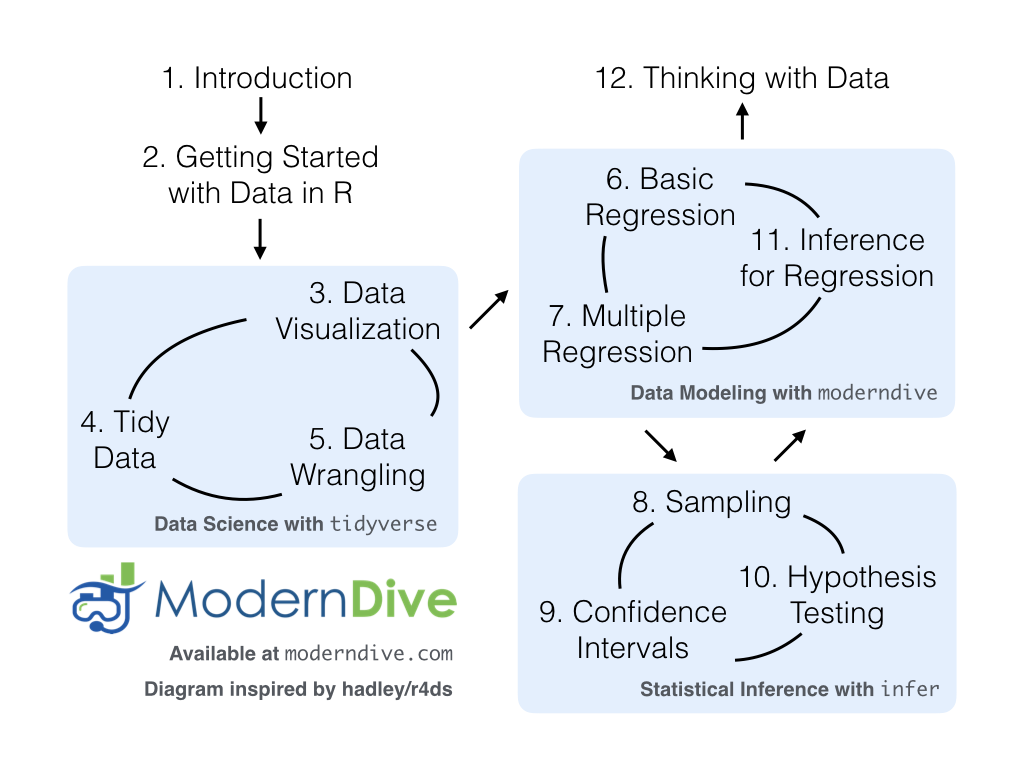
\includegraphics[width=\textwidth]{images/flowcharts/flowchart/flowchart.002} 

}

\caption{ModernDive Flowchart}\label{fig:moderndive-figure}
\end{figure}

\hypertarget{subsec:learning-goals}{%
\subsection{What you will learn from this book}\label{subsec:learning-goals}}

I hope that by the end of this book, you'll have learned

\begin{enumerate}
\def\labelenumi{\arabic{enumi}.}
\tightlist
\item
  How to use R to explore data.\\
\item
  How to answer statistical questions using tools like confidence intervals and hypothesis tests.
\item
  How to effectively create ``data stories'' using these tools.
\end{enumerate}

What do I mean by data stories? I mean any analysis involving data that engages the reader in answering questions with careful visuals and thoughtful discussion, such as \href{http://rpubs.com/ry_lisa_elana/chicago}{How strong is the relationship between per capita income and crime in Chicago neighborhoods?} and \href{https://ismayc.github.io/soc301_s2017/group_projects/group4.html}{How many f**ks does Quentin Tarantino give (as measured by the amount of swearing in his films)?}. Further discussions on data stories can be found in this \href{https://www.thinkwithgoogle.com/marketing-resources/data-measurement/tell-meaningful-stories-with-data/}{Think With Google article}.

For other examples of data stories constructed by students like yourselves, look at the final projects for two courses that have previously used ModernDive:

\begin{itemize}
\tightlist
\item
  Middlebury College \href{https://rudeboybert.github.io/MATH116/PS/final_project/final_project_outline.html\#past_examples}{MATH 116 Introduction to Statistical and Data Sciences} using student collected data.
\item
  Pacific University \href{https://ismayc.github.io/soc301_s2017/group-projects/index.html}{SOC 301 Social Statistics} using data from the \href{https://cran.r-project.org/web/packages/fivethirtyeight/vignettes/fivethirtyeight.html}{fivethirtyeight R package}.
\end{itemize}

This book will help you develop your ``data science toolbox'', including tools such as data visualization, data formatting, data wrangling, and data modeling using regression. With these tools, you'll be able to perform the entirety of the ``data/science pipeline'' while building data communication skills (see Subsection \ref{subsec:pipeline} for more details).

In particular, this book will lean heavily on data visualization. In today's world, we are bombarded with graphics that attempt to convey ideas. I will explore what makes a good graphic and what the standard ways are to convey relationships with data. You'll also see the use of visualization to introduce concepts like mean, median, standard deviation, distributions, etc. In general, I'll use visualization as a way of building almost all of the ideas in this book.

To impart the statistical lessons in this book, I have intentionally minimized the number of mathematical formulas used and instead have focused on developing a conceptual understanding via data visualization, statistical computing, and simulations. I hope this is a more intuitive experience than the way statistics has traditionally been taught in the past and how it is commonly perceived.

Finally, you'll learn the importance of literate programming. By this I mean you'll learn how to write code that is useful not just for a computer to execute but also for readers to understand exactly what your analysis is doing and how you did it. This is part of a greater effort to encourage reproducible research (see Subsection \ref{subsec:reproducible} for more details). Hal Abelson coined the phrase that I will follow throughout this book:

\begin{quote}
``Programs must be written for people to read, and only incidentally for machines to execute.''
\end{quote}

I understand that there may be challenging moments as you learn to program. Both of us continue to struggle and find ourselves often using web searches to find answers and reach out to colleagues for help. In the long run though, we all can solve problems faster and more elegantly via programming. I wrote this book as our way to help you get started and you should know that there is a huge community of R users that are always happy to help everyone along as well. This community exists in particular on the internet on various forums and websites such as \href{https://stackoverflow.com/}{stackoverflow.com}.

\hypertarget{subsec:pipeline}{%
\subsection{Data/science pipeline}\label{subsec:pipeline}}

You may think of statistics as just being a bunch of numbers. I commonly hear the phrase ``statistician'' when listening to broadcasts of sporting events. Statistics (in particular, data analysis), in addition to describing numbers like with baseball batting averages, plays a vital role in all of the sciences. You'll commonly hear the phrase ``statistically significant'' thrown around in the media. You'll see articles that say ``Science now shows that chocolate is good for you.'' Underpinning these claims is data analysis. By the end of this book, you'll be able to better understand whether these claims should be trusted or whether we should be wary. Inside data analysis are many sub-fields that I will discuss throughout this book (though not necessarily in this order):

\begin{itemize}
\tightlist
\item
  data collection
\item
  data wrangling
\item
  data visualization
\item
  data modeling
\item
  inference
\item
  correlation and regression
\item
  interpretation of results
\item
  data communication/storytelling
\end{itemize}

These sub-fields are summarized in what Grolemund and Wickham term the \href{http://r4ds.had.co.nz/explore-intro.html}{``Data/Science Pipeline''} in Figure \ref{fig:pipeline-figure}.

\begin{figure}

{\centering 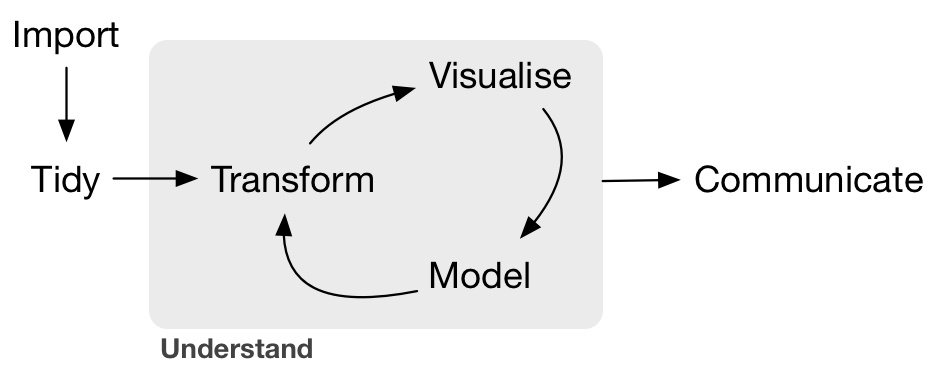
\includegraphics[width=\textwidth]{images/tidy1} 

}

\caption{Data/Science Pipeline}\label{fig:pipeline-figure}
\end{figure}

I will begin by digging into the gray \textbf{Understand} portion of the cycle with data visualization, then with a discussion on what is meant by tidy data and data wrangling, and then conclude by talking about interpreting and discussing the results of our models via \textbf{Communication}. These steps are vital to any statistical analysis. But why should you care about statistics? ``Why did they make me take this class?''

There's a reason so many fields require a statistics course. Scientific knowledge grows through an understanding of statistical significance and data analysis. You needn't be intimidated by statistics. It's not the beast that it used to be and, paired with computation, you'll see how reproducible research in the sciences particularly increases scientific knowledge.

\hypertarget{subsec:reproducible}{%
\subsection{Reproducible research}\label{subsec:reproducible}}

\begin{quote}
``The most important tool is the \emph{mindset}, when starting, that the end product will be reproducible.'' -- Keith Baggerly
\end{quote}

Another goal of this book is to help readers understand the importance of reproducible analyses. The hope is to get readers into the habit of making their analyses reproducible from the very beginning. This means I'll be trying to help you build new habits. This will take practice and be difficult at times. You'll see just why it is so important for you to keep track of your code and well-document it to help yourself later and any potential collaborators as well.

Copying and pasting results from one program into a word processor is not the way that efficient and effective scientific research is conducted. It's much more important for time to be spent on data collection and data analysis and not on copying and pasting plots back and forth across a variety of programs.

In a traditional analyses if an error was made with the original data, we'd need to step through the entire process again: recreate the plots and copy and paste all of the new plots and our statistical analysis into your document. This is error prone and a frustrating use of time. I'll see how to use R Markdown to get away from this tedious activity so that we can spend more time doing science.

\begin{quote}
``We are talking about \emph{computational} reproducibility.'' - Yihui Xie
\end{quote}

Reproducibility means a lot of things in terms of different scientific fields. Are experiments conducted in a way that another researcher could follow the steps and get similar results? In this book, I will focus on what is known as \textbf{computational reproducibility}. This refers to being able to pass all of one's data analysis, data-sets, and conclusions to someone else and have them get exactly the same results on their machine. This allows for time to be spent interpreting results and considering assumptions instead of the more error prone way of starting from scratch or following a list of steps that may be different from machine to machine.

\hypertarget{final-note-for-students}{%
\subsection{Final note for students}\label{final-note-for-students}}

At this point, if you are interested in instructor perspectives on this book, ways to contribute and collaborate, or the technical details of this book's construction and publishing, then continue with the rest of the chapter below. Otherwise, let's get started with R and RStudio in Chapter \ref{getting-started}!

\begin{center}\rule{0.5\linewidth}{\linethickness}\end{center}

\hypertarget{sec:intro-instructors}{%
\section{Introduction for instructors}\label{sec:intro-instructors}}

This book is inspired by the following books:

\begin{itemize}
\tightlist
\item
  ``Mathematical Statistics with Resampling and R'' \citep{hester2011},
\item
  ``OpenIntro: Intro Stat with Randomization and Simulation'' \citep{isrs2014}, and
\item
  ``R for Data Science'' \citep{rds2016}.
\end{itemize}

The first book, while designed for upper-level undergraduates and graduate students, provides an excellent resource on how to use resampling to impart statistical concepts like sampling distributions using computation instead of large-sample approximations and other mathematical formulas. The last two books are free options to learning introductory statistics and data science, providing an alternative to the many traditionally expensive introductory statistics textbooks.

When looking over the large number of introductory statistics textbooks that currently exist, I found that there wasn't one that incorporated many newly developed R packages directly into the text, in particular the many packages included in the \href{http://tidyverse.org/}{\texttt{tidyverse}} collection of packages, such as \texttt{ggplot2}, \texttt{dplyr}, \texttt{tidyr}, and \texttt{broom}. Additionally, there wasn't an open-source and easily reproducible textbook available that exposed new learners all of three of the learning goals listed at the outset of Subsection \ref{subsec:learning-goals}.

\hypertarget{who-is-this-book-for}{%
\subsection{Who is this book for?}\label{who-is-this-book-for}}

This book is intended for instructors of traditional introductory statistics classes using RStudio, either the desktop or server version, who would like to inject more data science topics into their syllabus. I assume that students taking the class will have no prior algebra, calculus, nor programming/coding experience.

Here are some principles and beliefs I kept in mind while writing this text. If you agree with them, this might be the book for you.

\begin{enumerate}
\def\labelenumi{\arabic{enumi}.}
\tightlist
\item
  \textbf{Blur the lines between lecture and lab}

  \begin{itemize}
  \tightlist
  \item
    With increased availability and accessibility of laptops and open-source non-proprietary statistical software, the strict dichotomy between lab and lecture can be loosened.
  \item
    It's much harder for students to understand the importance of using software if they only use it once a week or less. They forget the syntax in much the same way someone learning a foreign language forgets the rules. Frequent reinforcement is key.
  \end{itemize}
\item
  \textbf{Focus on the entire data/science research pipeline}

  \begin{itemize}
  \tightlist
  \item
    I believe that the entirety of Grolemund and Wickham's \href{http://r4ds.had.co.nz/introduction.html}{data/science pipeline} should be taught.
  \item
    I believe in \href{https://arxiv.org/abs/1507.05346}{``minimizing prerequisites to research''}: students should be answering questions with data as soon as possible.
  \end{itemize}
\item
  \textbf{It's all about the data}

  \begin{itemize}
  \tightlist
  \item
    I leverage R packages for rich, real, and realistic data-sets that at the same time are easy-to-load into R, such as the \texttt{nycflights13} and \texttt{fivethirtyeight} packages.
  \item
    I believe that \href{http://escholarship.org/uc/item/84v3774z}{data visualization is a gateway drug for statistics} and that the Grammar of Graphics as implemented in the \texttt{ggplot2} package is the best way to impart such lessons. However, I often hear: ``You can't teach \texttt{ggplot2} for data visualization in intro stats!'' I, like \href{http://varianceexplained.org/r/teach_ggplot2_to_beginners/}{David Robinson}, are much more optimistic.
  \item
    \texttt{dplyr} has made data wrangling much more \href{http://chance.amstat.org/2015/04/setting-the-stage/}{accessible} to novices, and hence much more interesting data-sets can be explored.
  \end{itemize}
\item
  \textbf{Use simulation/resampling to introduce statistical inference, not probability/mathematical formulas}

  \begin{itemize}
  \tightlist
  \item
    Instead of using formulas, large-sample approximations, and probability tables, statistical concepts using resampling-based inference.
  \item
    This allows for a de-emphasis of traditional probability topics, freeing up room in the syllabus for other topics.
  \end{itemize}
\item
  \textbf{Early exposure to analytics and computing}

  \begin{itemize}
  \tightlist
  \item
    Computing skills are essential to working with data in the 21st century even for HR managers. Given this fact, I feel that an early exposure to computing can only be of benefit to the whole HR community.
  \item
    I am not teaching a course on coding/programming per se, but rather just enough of the computational and algorithmic thinking necessary for performing a data analysis in HR.
  \end{itemize}
\item
  \textbf{Complete reproducibility and customisability}

  \begin{itemize}
  \tightlist
  \item
    I am frustrated when people talk about HR Analytics, without giving the source code and the data itself. I give you the source code for all examples as well as the whole book!
  \item
    If you want you can even use my book as a starting point and customise for your own non-profit training. For more about how to make this book your own, see \protect\hyperlink{sec:about-book}{About this Book}.
  \end{itemize}
\end{enumerate}

\begin{center}\rule{0.5\linewidth}{\linethickness}\end{center}

\hypertarget{sec:connect-contribute}{%
\section{Connect and contribute}\label{sec:connect-contribute}}

If you would like to connect with ``HR Analytics in R'', check out the following links:

\begin{itemize}
\tightlist
\item
  If you would like to receive periodic updates about HR Analytics, then please sign up for my \href{https://hranalytics.live/signup/}{mailing list}. You will receive receive bi-weekly notififications about my new blog posts.
\item
  Please feel free to contact me at \href{mailto:info@hranalytics.live}{\nolinkurl{info@hranalytics.live}} .
\item
  I am on Twitter at \href{https://twitter.com/h_feddersen}{h\_feddersen}.
\end{itemize}

If you would like to contribute to ``HR Analytics in R'', there are many ways! Let's all work together to make this book as great as possible for as many students as possible!

\begin{itemize}
\tightlist
\item
  Please let me know if you find any errors, typos, or areas from improvement on my \href{https://github.com/Hendrik147/HR_Analytics_in_R_book/issues}{GitHub issue page} page. I will fix it as soon as possible.
\item
  If you are familiar with GitHub and would like to contribute even more, please see Section \ref{sec:about-book} below.
\end{itemize}

I would like to thank \href{https://github.com/moderndive/moderndive_book}{Moderndive} for their inspirational presentation at a recent R user conference and for their generous example on how to set up a bookdown book and for their introductory pages on how to start using R.

\begin{center}\rule{0.5\linewidth}{\linethickness}\end{center}

\hypertarget{sec:about-book}{%
\section{About this book}\label{sec:about-book}}

This book was written using RStudio's \href{https://bookdown.org/}{bookdown} package by Yihui Xie \citep{R-bookdown}. This package simplifies the publishing of books by having all content written in \href{http://rmarkdown.rstudio.com/html_document_format.html}{R Markdown}.

\begin{itemize}
\item
  \textbf{Latest published version, still in development} The most up-to-date version, which is still in development is available at \url{https://hranalyticslive.netlify.com/}
\item
  \textbf{Source code} The bookdown/R Markdown source code for the latest version of ``HR Analytics in R'' is available on Hendrik Feddersen's \href{https://github.com/Hendrik147/HR_Analytics_in_R_book}{GitHub repository page}
\item
  \textbf{Usage} You can share this material with colleagues or for non-commercial purposes but you can't resell or incorporate them into stuff you make money from.

  \begin{itemize}
  \tightlist
  \item
    As a symbol of gratitude, I would expect you at least to sign up for my \href{https://hranalytics.live/signup/}{mailing list}.
  \item
    If you think my material is awesome and want to use it for commercial purposes, please contact me at \href{mailto:info@hranalytics.live}{\nolinkurl{info@hranalytics.live}}
  \end{itemize}
\item
  \textbf{Licence} This work is licensed under a Creative Commons
  Attribution-NonCommercial 4.0 International License.

  \begin{figure}
  \centering
  
\includegraphics{images/by-nc-sa.png}
  \caption{Creative Commons License}
  \end{figure}
\end{itemize}

\begin{center}\rule{0.5\linewidth}{\linethickness}\end{center}

\hypertarget{sec:about-authors}{%
\section{About the author}\label{sec:about-authors}}

Who am I?

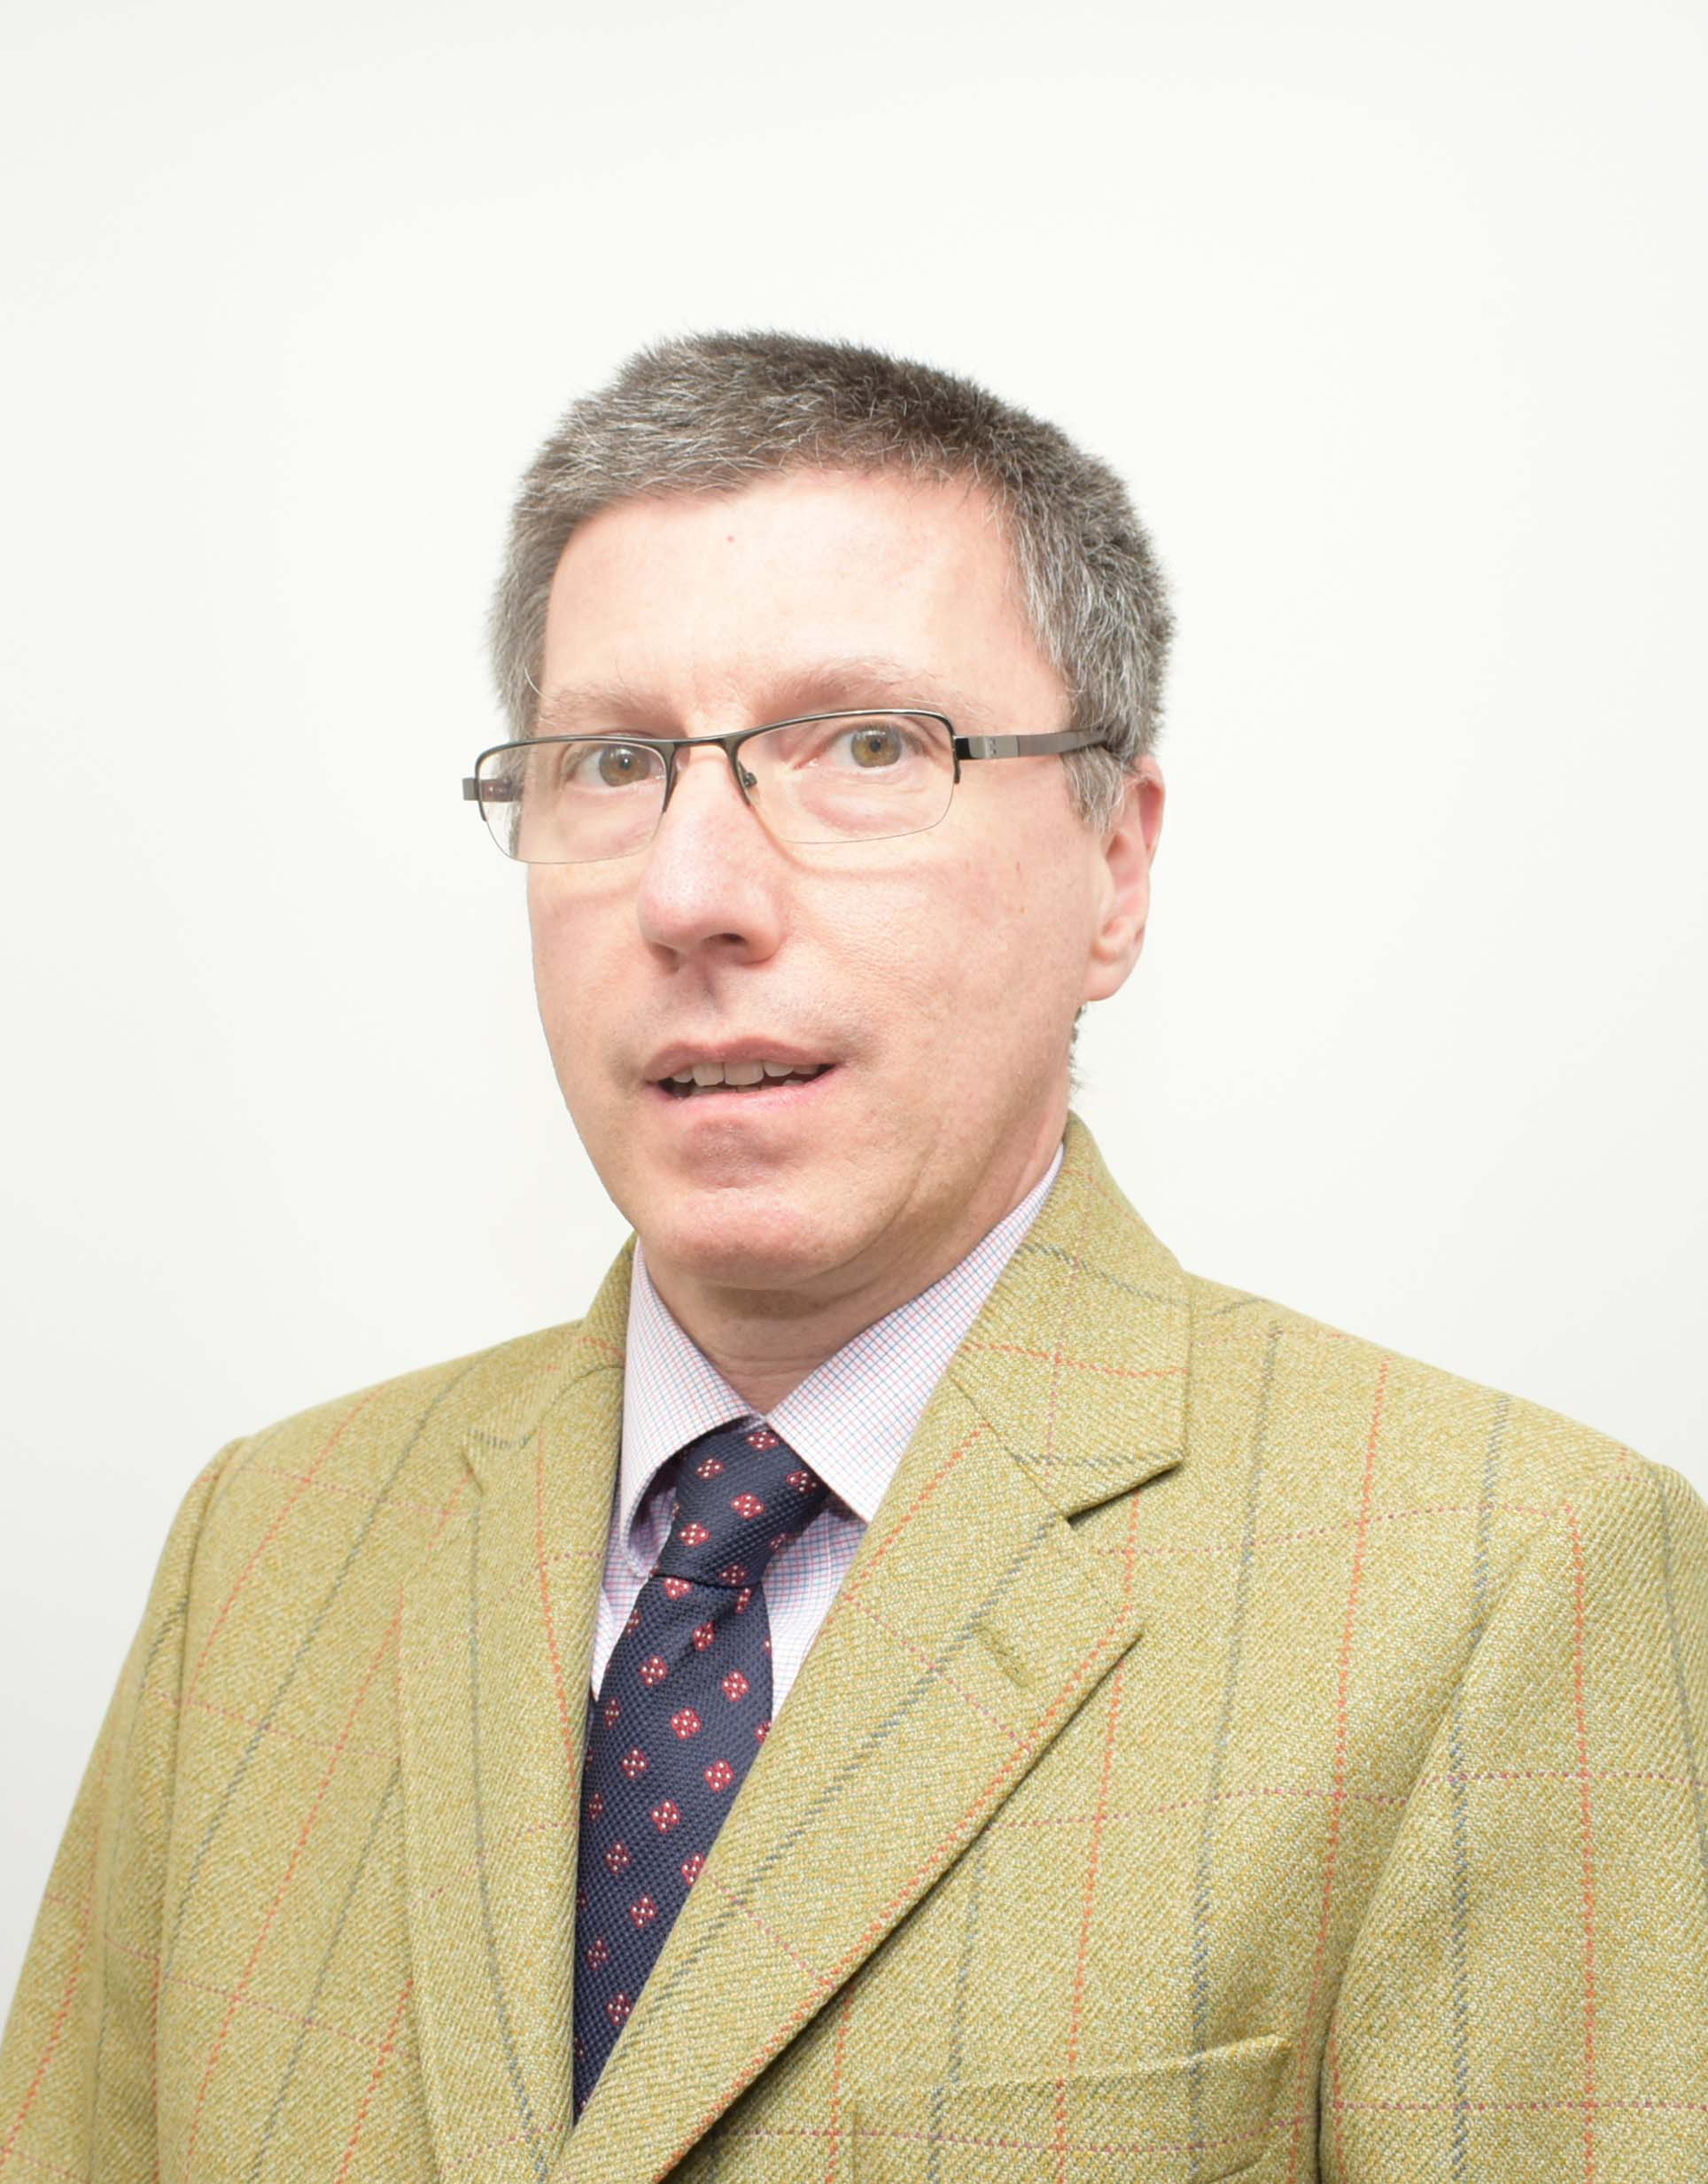
\includegraphics[width=0.4\textwidth,height=\textheight]{images/Photo HF Snappy.jpg}

\begin{itemize}
\item
  I am Hendrik Feddersen, a long-standing HR practitioner passionate about HR Analytics and living in Amsterdam, Netherlands.

  \begin{itemize}
  \tightlist
  \item
    Email: \href{mailto:info@hranalytics.live}{\nolinkurl{info@hranalytics.live}}
  \item
    Webpage: \url{https://hranalytics.live/}
  \item
    Twitter: \href{https://twitter.com/h_feddersen}{h\_feddersen}
  \item
    GitHub: \url{https://github.com/Hendrik147}
  \end{itemize}
\end{itemize}

\hypertarget{getting-started}{%
\chapter{Getting Started with Data in R}\label{getting-started}}

Placeholder

\hypertarget{r-rstudio}{%
\section{What are R and RStudio?}\label{r-rstudio}}

\hypertarget{installing-r-and-rstudio}{%
\subsection{Installing R and RStudio}\label{installing-r-and-rstudio}}

\hypertarget{using-r-via-rstudio}{%
\subsection{Using R via RStudio}\label{using-r-via-rstudio}}

\hypertarget{code}{%
\section{How do I code in R?}\label{code}}

\hypertarget{programming-concepts}{%
\subsection{Basic programming concepts and terminology}\label{programming-concepts}}

\hypertarget{errors-warnings-and-messages}{%
\subsection{Errors, warnings, and messages}\label{errors-warnings-and-messages}}

\hypertarget{tips-on-learning-to-code}{%
\subsection{Tips on learning to code}\label{tips-on-learning-to-code}}

\hypertarget{packages}{%
\section{What are R packages?}\label{packages}}

\hypertarget{package-installation}{%
\subsection{Package installation}\label{package-installation}}

\hypertarget{package-loading}{%
\subsection{Package loading}\label{package-loading}}

\hypertarget{package-use}{%
\subsection{Package use}\label{package-use}}

\hypertarget{nycflights13}{%
\section{Explore your first datasets}\label{nycflights13}}

\hypertarget{nycflights13-package}{%
\subsection{\texorpdfstring{\texttt{nycflights13} package}{nycflights13 package}}\label{nycflights13-package}}

\hypertarget{flights-data-frame}{%
\subsection{\texorpdfstring{\texttt{flights} data frame}{flights data frame}}\label{flights-data-frame}}

\hypertarget{exploredataframes}{%
\subsection{Exploring data frames}\label{exploredataframes}}

\hypertarget{identification-vs-measurement-variables}{%
\subsection{Identification \& measurement variables}\label{identification-vs-measurement-variables}}

\hypertarget{help-files}{%
\subsection{Help files}\label{help-files}}

\hypertarget{conclusion}{%
\section{Conclusion}\label{conclusion}}

\hypertarget{additional-resources}{%
\subsection{Additional resources}\label{additional-resources}}

\hypertarget{whats-to-come}{%
\subsection{What's to come?}\label{whats-to-come}}

\hypertarget{part-data-science-via-the-tidyverse}{%
\part{Data Science via the tidyverse}\label{part-data-science-via-the-tidyverse}}

\hypertarget{viz}{%
\chapter{Data Visualization}\label{viz}}

Placeholder

\hypertarget{needed-packages}{%
\subsection*{Needed packages}\label{needed-packages}}


\hypertarget{grammarofgraphics}{%
\section{The Grammar of Graphics}\label{grammarofgraphics}}

\hypertarget{components-of-the-grammar}{%
\subsection{Components of the Grammar}\label{components-of-the-grammar}}

\hypertarget{gapminder}{%
\subsection{Gapminder data}\label{gapminder}}

\hypertarget{other-components}{%
\subsection{Other components}\label{other-components}}

\hypertarget{ggplot2-package}{%
\subsection{ggplot2 package}\label{ggplot2-package}}

\hypertarget{FiveNG}{%
\section{Five Named Graphs - The 5NG}\label{FiveNG}}

\hypertarget{scatterplots}{%
\section{5NG\#1: Scatterplots}\label{scatterplots}}

\hypertarget{geompoint}{%
\subsection{Scatterplots via geom\_point}\label{geompoint}}

\hypertarget{overplotting}{%
\subsection{Over-plotting}\label{overplotting}}

\hypertarget{summary}{%
\subsection{Summary}\label{summary}}

\hypertarget{linegraphs}{%
\section{5NG\#2: Linegraphs}\label{linegraphs}}

\hypertarget{geomline}{%
\subsection{Linegraphs via geom\_line}\label{geomline}}

\hypertarget{summary-1}{%
\subsection{Summary}\label{summary-1}}

\hypertarget{histograms}{%
\section{5NG\#3: Histograms}\label{histograms}}

\hypertarget{geomhistogram}{%
\subsection{Histograms via geom\_histogram}\label{geomhistogram}}

\hypertarget{adjustbins}{%
\subsection{Adjusting the bins}\label{adjustbins}}

\hypertarget{summary-2}{%
\subsection{Summary}\label{summary-2}}

\hypertarget{facets}{%
\section{Facets}\label{facets}}

\hypertarget{boxplots}{%
\section{5NG\#4: Boxplots}\label{boxplots}}

\hypertarget{geomboxplot}{%
\subsection{Boxplots via geom\_boxplot}\label{geomboxplot}}

\hypertarget{summary-3}{%
\subsection{Summary}\label{summary-3}}

\hypertarget{geombar}{%
\section{5NG\#5: Barplots}\label{geombar}}

\hypertarget{barplots-via-geom_bar-or-geom_col}{%
\subsection{Barplots via geom\_bar or geom\_col}\label{barplots-via-geom_bar-or-geom_col}}

\hypertarget{must-avoid-pie-charts}{%
\subsection{Must avoid pie charts!}\label{must-avoid-pie-charts}}

\hypertarget{two-categ-barplot}{%
\subsection{Two categorical variables}\label{two-categ-barplot}}

\hypertarget{summary-4}{%
\subsection{Summary}\label{summary-4}}

\hypertarget{conclusion-1}{%
\section{Conclusion}\label{conclusion-1}}

\hypertarget{summary-table}{%
\subsection{Summary table}\label{summary-table}}

\hypertarget{argument-specification}{%
\subsection{Argument specification}\label{argument-specification}}

\hypertarget{additional-resources-1}{%
\subsection{Additional resources}\label{additional-resources-1}}

\hypertarget{whats-to-come-3}{%
\subsection{What's to come}\label{whats-to-come-3}}

\hypertarget{wrangling}{%
\chapter{Data Wrangling}\label{wrangling}}

Placeholder

\hypertarget{needed-packages-1}{%
\subsection*{Needed packages}\label{needed-packages-1}}


\hypertarget{piping}{%
\section{\texorpdfstring{The pipe operator: \texttt{\%\textgreater{}\%}}{The pipe operator: \%\textgreater\%}}\label{piping}}

\hypertarget{filter}{%
\section{\texorpdfstring{\texttt{filter} rows}{filter rows}}\label{filter}}

\hypertarget{summarize}{%
\section{\texorpdfstring{\texttt{summarize} variables}{summarize variables}}\label{summarize}}

\hypertarget{groupby}{%
\section{\texorpdfstring{\texttt{group\_by} rows}{group\_by rows}}\label{groupby}}

\hypertarget{grouping-by-more-than-one-variable}{%
\subsection{Grouping by more than one variable}\label{grouping-by-more-than-one-variable}}

\hypertarget{mutate}{%
\section{\texorpdfstring{\texttt{mutate} existing variables}{mutate existing variables}}\label{mutate}}

\hypertarget{arrange}{%
\section{\texorpdfstring{\texttt{arrange} and sort rows}{arrange and sort rows}}\label{arrange}}

\hypertarget{joins}{%
\section{\texorpdfstring{\texttt{join} data frames}{join data frames}}\label{joins}}

\hypertarget{matching-key-variable-names}{%
\subsection{Matching ``key'' variable names}\label{matching-key-variable-names}}

\hypertarget{diff-key}{%
\subsection{Different ``key'' variable names}\label{diff-key}}

\hypertarget{multiple-key-variables}{%
\subsection{Multiple ``key'' variables}\label{multiple-key-variables}}

\hypertarget{normal-forms}{%
\subsection{Normal forms}\label{normal-forms}}

\hypertarget{other-verbs}{%
\section{Other verbs}\label{other-verbs}}

\hypertarget{select}{%
\subsection{\texorpdfstring{\texttt{select} variables}{select variables}}\label{select}}

\hypertarget{rename}{%
\subsection{\texorpdfstring{\texttt{rename} variables}{rename variables}}\label{rename}}

\hypertarget{top_n-values-of-a-variable}{%
\subsection{\texorpdfstring{\texttt{top\_n} values of a variable}{top\_n values of a variable}}\label{top_n-values-of-a-variable}}

\hypertarget{conclusion-2}{%
\section{Conclusion}\label{conclusion-2}}

\hypertarget{summary-table-1}{%
\subsection{Summary table}\label{summary-table-1}}

\hypertarget{additional-resources-2}{%
\subsection{Additional resources}\label{additional-resources-2}}

\hypertarget{whats-to-come-1}{%
\subsection{What's to come?}\label{whats-to-come-1}}

\hypertarget{tidy}{%
\chapter{Data Importing \& ``Tidy'' Data}\label{tidy}}

Placeholder

\hypertarget{needed-packages-2}{%
\subsection*{Needed packages}\label{needed-packages-2}}


\hypertarget{csv}{%
\section{Importing data}\label{csv}}

\hypertarget{using-the-console}{%
\subsection{Using the console}\label{using-the-console}}

\hypertarget{using-rstudios-interface}{%
\subsection{Using RStudio's interface}\label{using-rstudios-interface}}

\hypertarget{tidy-data-ex}{%
\section{Tidy data}\label{tidy-data-ex}}

\hypertarget{definition-of-tidy-data}{%
\subsection{Definition of ``tidy'' data}\label{definition-of-tidy-data}}

\hypertarget{converting-to-tidy-data}{%
\subsection{Converting to ``tidy'' data}\label{converting-to-tidy-data}}

\hypertarget{nycflights13-package-1}{%
\subsection{\texorpdfstring{\texttt{nycflights13} package}{nycflights13 package}}\label{nycflights13-package-1}}

\hypertarget{case-study-tidy}{%
\section{Case study: Democracy in Guatemala}\label{case-study-tidy}}

\hypertarget{conclusion-3}{%
\section{Conclusion}\label{conclusion-3}}

\hypertarget{tidyverse-package}{%
\subsection{\texorpdfstring{\texttt{tidyverse} package}{tidyverse package}}\label{tidyverse-package}}

\hypertarget{additional-resources-3}{%
\subsection{Additional resources}\label{additional-resources-3}}

\hypertarget{whats-to-come-2}{%
\subsection{What's to come?}\label{whats-to-come-2}}

\hypertarget{part-data-modeling-via-moderndive}{%
\part{Data Modeling via moderndive}\label{part-data-modeling-via-moderndive}}

\hypertarget{regression}{%
\chapter{Basic Regression}\label{regression}}

Placeholder

\hypertarget{needed-packages-3}{%
\subsection*{Needed packages}\label{needed-packages-3}}


\hypertarget{model1}{%
\section{One numerical explanatory variable}\label{model1}}

\hypertarget{model1EDA}{%
\subsection{Exploratory data analysis}\label{model1EDA}}

\hypertarget{model1table}{%
\subsection{Simple linear regression}\label{model1table}}

\hypertarget{model1points}{%
\subsection{Observed/fitted values and residuals}\label{model1points}}

\hypertarget{model2}{%
\section{One categorical explanatory variable}\label{model2}}

\hypertarget{model2EDA}{%
\subsection{Exploratory data analysis}\label{model2EDA}}

\hypertarget{model2table}{%
\subsection{Linear regression}\label{model2table}}

\hypertarget{model2points}{%
\subsection{Observed/fitted values and residuals}\label{model2points}}

\hypertarget{related-topics}{%
\section{Related topics}\label{related-topics}}

\hypertarget{correlation-is-not-causation}{%
\subsection{Correlation is not necessarily causation}\label{correlation-is-not-causation}}

\hypertarget{leastsquares}{%
\subsection{Best fitting line}\label{leastsquares}}

\hypertarget{underthehood}{%
\subsection{\texorpdfstring{\texttt{get\_regression\_x()} functions}{get\_regression\_x() functions}}\label{underthehood}}

\hypertarget{conclusion-4}{%
\section{Conclusion}\label{conclusion-4}}

\hypertarget{additional-resources-basic-regression}{%
\subsection{Additional resources}\label{additional-resources-basic-regression}}

\hypertarget{whats-to-come-4}{%
\subsection{What's to come?}\label{whats-to-come-4}}

\hypertarget{multiple-regression}{%
\chapter{Multiple Regression}\label{multiple-regression}}

Placeholder

\hypertarget{needed-packages-4}{%
\subsection*{Needed packages}\label{needed-packages-4}}


\hypertarget{model4}{%
\section{One numerical \& one categorical explanatory variable}\label{model4}}

\hypertarget{model4EDA}{%
\subsection{Exploratory data analysis}\label{model4EDA}}

\hypertarget{model4interactiontable}{%
\subsection{Interaction model}\label{model4interactiontable}}

\hypertarget{model4table}{%
\subsection{Parallel slopes model}\label{model4table}}

\hypertarget{model4points}{%
\subsection{Observed/fitted values and residuals}\label{model4points}}

\hypertarget{model3}{%
\section{Two numerical explanatory variables}\label{model3}}

\hypertarget{model3EDA}{%
\subsection{Exploratory data analysis}\label{model3EDA}}

\hypertarget{model3table}{%
\subsection{Regression plane}\label{model3table}}

\hypertarget{model3points}{%
\subsection{Observed/fitted values and residuals}\label{model3points}}

\hypertarget{related-topics-1}{%
\section{Related topics}\label{related-topics-1}}

\hypertarget{model-selection}{%
\subsection{Model selection}\label{model-selection}}

\hypertarget{correlationcoefficient2}{%
\subsection{Correlation coefficient}\label{correlationcoefficient2}}

\hypertarget{simpsonsparadox}{%
\subsection{Simpson's Paradox}\label{simpsonsparadox}}

\hypertarget{conclusion-5}{%
\section{Conclusion}\label{conclusion-5}}

\hypertarget{additional-resources-4}{%
\subsection{Additional resources}\label{additional-resources-4}}

\hypertarget{whats-to-come-5}{%
\subsection{What's to come?}\label{whats-to-come-5}}

\hypertarget{part-statistical-inference-via-infer}{%
\part{Statistical inference via infer}\label{part-statistical-inference-via-infer}}

\hypertarget{sampling}{%
\chapter{Sampling}\label{sampling}}

Placeholder

\hypertarget{needed-packages-5}{%
\subsection*{Needed packages}\label{needed-packages-5}}


\hypertarget{sampling-activity}{%
\section{Sampling activity}\label{sampling-activity}}

\hypertarget{what-proportion-of-this-bowls-balls-are-red}{%
\subsection{What proportion of this bowl's balls are red?}\label{what-proportion-of-this-bowls-balls-are-red}}

\hypertarget{using-the-shovel-once}{%
\subsection{Using the shovel once}\label{using-the-shovel-once}}

\hypertarget{student-shovels}{%
\subsection{Using the shovel 33 times}\label{student-shovels}}

\hypertarget{what-are-we-doing-here}{%
\subsection{What are we doing here?}\label{what-are-we-doing-here}}

\hypertarget{sampling-simulation}{%
\section{Computer simulation of sampling}\label{sampling-simulation}}

\hypertarget{using-the-virtual-shovel-once}{%
\subsection{Using the virtual shovel once}\label{using-the-virtual-shovel-once}}

\hypertarget{using-the-virtual-shovel-33-times}{%
\subsection{Using the virtual shovel 33 times}\label{using-the-virtual-shovel-33-times}}

\hypertarget{shovel-1000-times}{%
\subsection{Using the virtual shovel 1000 times}\label{shovel-1000-times}}

\hypertarget{different-shovels}{%
\subsection{Using different shovels}\label{different-shovels}}

\hypertarget{sampling-framework}{%
\section{Sampling framework}\label{sampling-framework}}

\hypertarget{terminology-and-notation}{%
\subsection{Terminology \& notation}\label{terminology-and-notation}}

\hypertarget{statistical-definitions}{%
\subsection{Statistical definitions}\label{statistical-definitions}}

\hypertarget{the-moral-of-the-story}{%
\subsection{The moral of the story}\label{the-moral-of-the-story}}

\hypertarget{sampling-case-study}{%
\section{Case study: Polls}\label{sampling-case-study}}

\hypertarget{sampling-conclusion}{%
\section{Conclusion}\label{sampling-conclusion}}

\hypertarget{sampling-conclusion-sampling-vs-assignment}{%
\subsection{Random sampling vs random assignment}\label{sampling-conclusion-sampling-vs-assignment}}

\hypertarget{sampling-conclusion-central-limit-theorem}{%
\subsection{Central Limit Theorem}\label{sampling-conclusion-central-limit-theorem}}

\hypertarget{sampling-conclusion-table}{%
\subsection{Summary table}\label{sampling-conclusion-table}}

\hypertarget{additional-resources-5}{%
\subsection{Additional resources}\label{additional-resources-5}}

\hypertarget{whats-to-come-6}{%
\subsection{What's to come?}\label{whats-to-come-6}}

\hypertarget{confidence-intervals}{%
\chapter{Confidence Intervals}\label{confidence-intervals}}

Placeholder

\hypertarget{needed-packages-6}{%
\subsection*{Needed packages}\label{needed-packages-6}}


\hypertarget{resampling-activity}{%
\section{Resampling activity}\label{resampling-activity}}

\hypertarget{what-is-the-average-year-of-circulated-us-pennies-in-2019}{%
\subsection{What is the average year of circulated US pennies in 2019?}\label{what-is-the-average-year-of-circulated-us-pennies-in-2019}}

\hypertarget{exploratory-data-analysis-on-original-sample}{%
\subsubsection*{Exploratory data analysis on original sample}\label{exploratory-data-analysis-on-original-sample}}


\hypertarget{using-resampling-once}{%
\subsection{Using resampling once}\label{using-resampling-once}}

\hypertarget{exploratory-data-analysis-on-the-resample}{%
\subsubsection*{Exploratory data analysis on the resample}\label{exploratory-data-analysis-on-the-resample}}


\hypertarget{student-resamples}{%
\subsection{Using resampling 33 times}\label{student-resamples}}

\hypertarget{whats-the-plan}{%
\subsection{What's the plan?}\label{whats-the-plan}}

\hypertarget{resampling-simulation}{%
\section{Computer simulation of resampling}\label{resampling-simulation}}

\hypertarget{using-the-virtual-resample-once}{%
\subsection{Using the virtual resample once}\label{using-the-virtual-resample-once}}

\hypertarget{using-the-virtual-resample-33-times}{%
\subsection{Using the virtual resample 33 times}\label{using-the-virtual-resample-33-times}}

\hypertarget{using-the-virtual-resample-1000-times}{%
\subsection{Using the virtual resample 1000 times}\label{using-the-virtual-resample-1000-times}}

\hypertarget{ci-build-up}{%
\section{Confidence interval build-up}\label{ci-build-up}}

\hypertarget{percentile-method}{%
\subsection{The percentile method}\label{percentile-method}}

\hypertarget{the-standard-error-method}{%
\subsection{The standard error method}\label{the-standard-error-method}}

\hypertarget{bootstrap-process}{%
\section{The bootstrapping framework}\label{bootstrap-process}}

\hypertarget{the-original-workflow-needed-for-this}{%
\subsection{The original workflow needed for this}\label{the-original-workflow-needed-for-this}}

\hypertarget{the-infer-package-for-statistical-inference}{%
\subsection{The infer package for statistical inference}\label{the-infer-package-for-statistical-inference}}

\hypertarget{specify-variables}{%
\subsubsection*{Specify variables}\label{specify-variables}}


\hypertarget{generate-replicates}{%
\subsubsection*{Generate replicates}\label{generate-replicates}}


\hypertarget{calculate-summary-statistics}{%
\subsubsection*{Calculate summary statistics}\label{calculate-summary-statistics}}


\hypertarget{observed-statistic-point-estimate-calculations}{%
\subsubsection*{Observed statistic / point estimate calculations}\label{observed-statistic-point-estimate-calculations}}


\hypertarget{visualize-the-results}{%
\subsubsection*{Visualize the results}\label{visualize-the-results}}


\hypertarget{infer-ci}{%
\subsection{Building confidence intervals with the infer package}\label{infer-ci}}

\hypertarget{percentile-method-infer}{%
\subsection{The percentile method with infer}\label{percentile-method-infer}}

\hypertarget{the-standard-error-method-with-infer}{%
\subsection{The standard error method with infer}\label{the-standard-error-method-with-infer}}

\hypertarget{one-prop-ci}{%
\section{Case study: Revisiting the red ball example}\label{one-prop-ci}}

\hypertarget{observed-statistic}{%
\subsection{Observed statistic}\label{observed-statistic}}

\hypertarget{one-prop-boot}{%
\subsection{Bootstrap distribution for one proportion}\label{one-prop-boot}}

\hypertarget{interpreting-the-confidence-interval}{%
\section{Interpreting the confidence interval}\label{interpreting-the-confidence-interval}}

\hypertarget{back-to-our-pennies-example}{%
\subsubsection*{Back to our pennies example}\label{back-to-our-pennies-example}}


\hypertarget{the-width-of-confidence-intervals}{%
\subsection*{The width of confidence intervals}\label{the-width-of-confidence-intervals}}


\hypertarget{the-impact-of-confidence-levels}{%
\subsubsection*{The impact of confidence levels}\label{the-impact-of-confidence-levels}}


\hypertarget{the-impact-of-sample-size}{%
\subsubsection*{The impact of sample size}\label{the-impact-of-sample-size}}


\hypertarget{case-study-two-prop-ci}{%
\section{Case study: Comparing two proportions}\label{case-study-two-prop-ci}}

\hypertarget{compute-the-point-estimate}{%
\subsection{Compute the point estimate}\label{compute-the-point-estimate}}

\hypertarget{bootstrap-distribution}{%
\subsection{Bootstrap distribution}\label{bootstrap-distribution}}

\hypertarget{ci-conclusion}{%
\section{Conclusion}\label{ci-conclusion}}

\hypertarget{comparing-bootstrap-and-sampling-distributions}{%
\subsection{Comparing bootstrap and sampling distributions}\label{comparing-bootstrap-and-sampling-distributions}}

\hypertarget{sampling-distribution}{%
\subsubsection*{Sampling distribution}\label{sampling-distribution}}


\hypertarget{bootstrap-distribution-1}{%
\subsubsection*{Bootstrap distribution}\label{bootstrap-distribution-1}}


\hypertarget{theory-ci}{%
\subsection{Theory-based confidence intervals}\label{theory-ci}}

\hypertarget{procedure-for-building-a-theory-based-ci-for-p}{%
\subsubsection*{\texorpdfstring{Procedure for building a theory-based CI for \(p\)}{Procedure for building a theory-based CI for p}}\label{procedure-for-building-a-theory-based-ci-for-p}}


\hypertarget{confidence-intervals-based-on-33-tactile-samples}{%
\subsubsection*{Confidence intervals based on 33 tactile samples}\label{confidence-intervals-based-on-33-tactile-samples}}


\hypertarget{confidence-intervals-based-on-100-virtual-samples}{%
\subsubsection*{Confidence intervals based on 100 virtual samples}\label{confidence-intervals-based-on-100-virtual-samples}}


\hypertarget{where-does-the-1.96-come-from}{%
\subsubsection*{Where does the 1.96 come from?}\label{where-does-the-1.96-come-from}}


\hypertarget{ci-conclusion-table}{%
\subsection{Summary table}\label{ci-conclusion-table}}

\hypertarget{additional-resources-6}{%
\subsection{Additional resources}\label{additional-resources-6}}

\hypertarget{whats-to-come-7}{%
\subsection{What's to come?}\label{whats-to-come-7}}

\hypertarget{hypothesis-testing}{%
\chapter{Hypothesis Testing}\label{hypothesis-testing}}

Placeholder

\hypertarget{needed-packages-7}{%
\subsection*{Needed packages}\label{needed-packages-7}}


\hypertarget{ht-activity}{%
\section{Hypothesis testing activity}\label{ht-activity}}

\hypertarget{question-of-interest}{%
\subsection{Question of interest}\label{question-of-interest}}

\hypertarget{what-did-we-actually-observe}{%
\subsection{What did we actually observe?}\label{what-did-we-actually-observe}}

\hypertarget{using-permuting-once}{%
\subsection{Using permuting once}\label{using-permuting-once}}

\hypertarget{using-permuting-33-times}{%
\subsection{Using permuting 33 times}\label{using-permuting-33-times}}

\hypertarget{ht-infer}{%
\section{Hypothesis testing with infer}\label{ht-infer}}

\hypertarget{revisiting-the-infer-verb-framework}{%
\subsection{Revisiting the infer verb framework}\label{revisiting-the-infer-verb-framework}}

\hypertarget{the-infer-pipeline-for-the-activity}{%
\subsection{\texorpdfstring{The \texttt{infer} pipeline for the activity}{The infer pipeline for the activity}}\label{the-infer-pipeline-for-the-activity}}

\hypertarget{choose-the-variables-of-interest}{%
\subsubsection*{Choose the variables of interest}\label{choose-the-variables-of-interest}}


\hypertarget{set-the-model-for-the-null-hypothesis}{%
\subsubsection*{Set the model for the null hypothesis}\label{set-the-model-for-the-null-hypothesis}}


\hypertarget{replicate-samples-assuming-the-null-hypothesis-is-true}{%
\subsubsection*{Replicate samples assuming the null hypothesis is true}\label{replicate-samples-assuming-the-null-hypothesis-is-true}}


\hypertarget{compute-the-statistic-for-each-replicate}{%
\subsubsection*{Compute the statistic for each replicate}\label{compute-the-statistic-for-each-replicate}}


\hypertarget{only-one-test}{%
\subsection{The ``There Is Only One Test'' framework}\label{only-one-test}}

\hypertarget{p-value}{%
\section{The p-value}\label{p-value}}

\hypertarget{corresponding-confidence-interval}{%
\subsection{Corresponding confidence interval}\label{corresponding-confidence-interval}}

\hypertarget{summary-5}{%
\subsection{Summary}\label{summary-5}}

\hypertarget{ht-interpretation}{%
\section{Interpretation of hypothesis testing results}\label{ht-interpretation}}

\hypertarget{trial}{%
\subsection{Criminal trial analogy}\label{trial}}

\hypertarget{two-possible-conclusions}{%
\subsubsection*{Two possible conclusions}\label{two-possible-conclusions}}


\hypertarget{types-of-errors-in-hypothesis-testing}{%
\subsection{Types of errors in hypothesis testing}\label{types-of-errors-in-hypothesis-testing}}

\hypertarget{logic-of-hypothesis-testing}{%
\subsubsection*{Logic of hypothesis testing}\label{logic-of-hypothesis-testing}}


\hypertarget{statistical-significance}{%
\subsection{Statistical significance}\label{statistical-significance}}

\hypertarget{ht-case-study}{%
\section{Case study: comparing two means}\label{ht-case-study}}

\hypertarget{randomizationpermutation}{%
\subsection{Randomization/permutation}\label{randomizationpermutation}}

\hypertarget{comparing-action-and-romance-movies}{%
\subsection{Comparing action and romance movies}\label{comparing-action-and-romance-movies}}

\hypertarget{sampling-rightarrow-randomization}{%
\subsection{\texorpdfstring{Sampling \(\rightarrow\) randomization}{Sampling \textbackslash rightarrow randomization}}\label{sampling-rightarrow-randomization}}

\hypertarget{data}{%
\subsection{Data}\label{data}}

\hypertarget{model-of-h_0}{%
\subsection{\texorpdfstring{Model of \(H_0\)}{Model of H\_0}}\label{model-of-h_0}}

\hypertarget{test-statistic-delta}{%
\subsection{\texorpdfstring{Test statistic \(\delta\)}{Test statistic \textbackslash delta}}\label{test-statistic-delta}}

\hypertarget{observed-effect-delta}{%
\subsection{\texorpdfstring{Observed effect \(\delta^*\)}{Observed effect \textbackslash delta\^{}*}}\label{observed-effect-delta}}

\hypertarget{simulated-data}{%
\subsection{Simulated data}\label{simulated-data}}

\hypertarget{distribution-of-delta-under-h_0}{%
\subsection{\texorpdfstring{Distribution of \(\delta\) under \(H_0\)}{Distribution of \textbackslash delta under H\_0}}\label{distribution-of-delta-under-h_0}}

\hypertarget{the-p-value}{%
\subsection{The p-value}\label{the-p-value}}

\hypertarget{corresponding-confidence-interval-1}{%
\subsection{Corresponding confidence interval}\label{corresponding-confidence-interval-1}}

\hypertarget{conclusion-6}{%
\section{Conclusion}\label{conclusion-6}}

\hypertarget{when-inference-is-not-needed}{%
\subsection{When inference is not needed}\label{when-inference-is-not-needed}}

\hypertarget{problems-with-p-values}{%
\subsection{Problems with p-values}\label{problems-with-p-values}}

\hypertarget{comparing-confidence-intervals-and-hypothesis-tests}{%
\subsection{Comparing confidence intervals and hypothesis tests}\label{comparing-confidence-intervals-and-hypothesis-tests}}

\hypertarget{ht-conclusion-table}{%
\subsection{Summary table}\label{ht-conclusion-table}}

\hypertarget{theory-hypo}{%
\subsection{Building theory-based methods using computation}\label{theory-hypo}}

\hypertarget{example-t-test-for-two-independent-samples}{%
\subsubsection*{\texorpdfstring{Example: \(t\)-test for two independent samples}{Example: t-test for two independent samples}}\label{example-t-test-for-two-independent-samples}}


\hypertarget{conditions-for-t-test}{%
\subsubsection*{Conditions for t-test}\label{conditions-for-t-test}}


\hypertarget{additional-resources-7}{%
\subsection{Additional resources}\label{additional-resources-7}}

\hypertarget{whats-to-come-8}{%
\subsection{What's to come}\label{whats-to-come-8}}

\hypertarget{inference-for-regression}{%
\chapter{Inference for Regression}\label{inference-for-regression}}

Placeholder

\hypertarget{needed-packages-8}{%
\subsection*{Needed packages}\label{needed-packages-8}}


\hypertarget{simulation-based-inference-for-regression}{%
\section{Simulation-based Inference for Regression}\label{simulation-based-inference-for-regression}}

\hypertarget{data-1}{%
\subsection{Data}\label{data-1}}

\hypertarget{test-statistic-delta-1}{%
\subsection{\texorpdfstring{Test statistic \(\delta\)}{Test statistic \textbackslash delta}}\label{test-statistic-delta-1}}

\hypertarget{observed-effect-delta-1}{%
\subsection{\texorpdfstring{Observed effect \(\delta^*\)}{Observed effect \textbackslash delta\^{}*}}\label{observed-effect-delta-1}}

\hypertarget{model-of-h_0-1}{%
\subsection{\texorpdfstring{Model of \(H_0\)}{Model of H\_0}}\label{model-of-h_0-1}}

\hypertarget{simulated-data-1}{%
\subsection{Simulated data}\label{simulated-data-1}}

\hypertarget{distribution-of-delta-under-h_0-1}{%
\subsection{\texorpdfstring{Distribution of \(\delta\) under \(H_0\)}{Distribution of \textbackslash delta under H\_0}}\label{distribution-of-delta-under-h_0-1}}

\hypertarget{the-p-value-1}{%
\subsection{The p-value}\label{the-p-value-1}}

\hypertarget{bootstrapping-for-the-regression-slope}{%
\section{Bootstrapping for the regression slope}\label{bootstrapping-for-the-regression-slope}}

\hypertarget{inference-for-multiple-regression}{%
\section{Inference for multiple regression}\label{inference-for-multiple-regression}}

\hypertarget{refresher-professor-evaluations-data}{%
\subsection{Refresher: Professor evaluations data}\label{refresher-professor-evaluations-data}}

\hypertarget{refresher-visualizations}{%
\subsection{Refresher: Visualizations}\label{refresher-visualizations}}

\hypertarget{refresher-regression-tables}{%
\subsection{Refresher: Regression tables}\label{refresher-regression-tables}}

\hypertarget{script-of-r-code}{%
\subsection{Script of R code}\label{script-of-r-code}}

\hypertarget{residual-analysis}{%
\section{Residual analysis}\label{residual-analysis}}

\hypertarget{model1residuals}{%
\subsection{Residual analysis}\label{model1residuals}}

\hypertarget{model2residuals}{%
\subsection{Residual analysis}\label{model2residuals}}

\hypertarget{model3residuals}{%
\subsection{Residual analysis}\label{model3residuals}}

\hypertarget{model4residuals}{%
\subsection{Residual analysis}\label{model4residuals}}

\hypertarget{part-learnings-so-far}{%
\part{Learnings so far}\label{part-learnings-so-far}}

\hypertarget{thinking-with-data}{%
\chapter{Thinking with Data}\label{thinking-with-data}}

Placeholder

\hypertarget{needed-packages-9}{%
\subsection*{Needed packages}\label{needed-packages-9}}


\hypertarget{seattle-house-prices}{%
\section{Case study: Seattle house prices}\label{seattle-house-prices}}

\hypertarget{house-prices-EDA-I}{%
\subsection{Exploratory data analysis (EDA)}\label{house-prices-EDA-I}}

\hypertarget{log10-transformations}{%
\subsection{log10 transformations}\label{log10-transformations}}

\hypertarget{eda-part-ii}{%
\subsection{EDA Part II}\label{eda-part-ii}}

\hypertarget{house-prices-regression}{%
\subsection{Regression modeling}\label{house-prices-regression}}

\hypertarget{house-prices-inference-for-regression}{%
\subsection{Inference for regression}\label{house-prices-inference-for-regression}}

\hypertarget{house-prices-making-predictions}{%
\subsection{Making predictions}\label{house-prices-making-predictions}}

\hypertarget{data-journalism}{%
\section{Case study: Effective data storytelling}\label{data-journalism}}

\hypertarget{bechdel-test-for-hollywood-gender-representation}{%
\subsection{Bechdel test for Hollywood gender representation}\label{bechdel-test-for-hollywood-gender-representation}}

\hypertarget{us-births-in-1999}{%
\subsection{US Births in 1999}\label{us-births-in-1999}}

\hypertarget{other-examples}{%
\subsection{Other examples}\label{other-examples}}

\hypertarget{script-of-r-code-1}{%
\subsection{Script of R code}\label{script-of-r-code-1}}

\hypertarget{concluding-remarks}{%
\section*{Concluding remarks}\label{concluding-remarks}}


\hypertarget{part-practical-examples-about-hr-analytics}{%
\part{Practical examples about HR Analytics}\label{part-practical-examples-about-hr-analytics}}

\hypertarget{pay-gap}{%
\chapter{Gender Pay Gap}\label{pay-gap}}

Placeholder

\hypertarget{data-cleaning-and-prep.}{%
\section{Data Cleaning and Prep.}\label{data-cleaning-and-prep.}}

\hypertarget{summary-statistics-by-gender}{%
\section{Summary Statistics by gender}\label{summary-statistics-by-gender}}

\hypertarget{avoiding-simpsons-paradox}{%
\section{Avoiding Simpson's Paradox}\label{avoiding-simpsons-paradox}}

\hypertarget{model-estimation-ols-with-controls.}{%
\section{Model Estimation: OLS with controls.}\label{model-estimation-ols-with-controls.}}

\hypertarget{logarithm-of-base-pay}{%
\subsection{Logarithm of Base Pay}\label{logarithm-of-base-pay}}

\hypertarget{results-by-department}{%
\subsection{Results by Department}\label{results-by-department}}

\hypertarget{results-by-job-title}{%
\subsection{Results by Job Title}\label{results-by-job-title}}

\hypertarget{stop-appraisals}{%
\chapter{Stop the formal performance management process}\label{stop-appraisals}}

Placeholder

\hypertarget{service-desk}{%
\chapter{HR Service Desk}\label{service-desk}}

Placeholder

\hypertarget{personality}{%
\chapter{Personality insights}\label{personality}}

Placeholder

\hypertarget{commuting-time}{%
\chapter{Commuting time}\label{commuting-time}}

Placeholder

\hypertarget{orgnisational-network}{%
\chapter{Module - Organisational network analysis}\label{orgnisational-network}}

Placeholder

\hypertarget{job-classification}{%
\chapter{Job classification analysis}\label{job-classification}}

Placeholder

\hypertarget{final-evaluation-of-the-various-models}{%
\subsection{Final evaluation of the various models}\label{final-evaluation-of-the-various-models}}

\hypertarget{masking-data}{%
\chapter{Masking HR data}\label{masking-data}}

Placeholder

\hypertarget{whitehouse-dataset}{%
\subsection{Whitehouse dataset}\label{whitehouse-dataset}}

\hypertarget{fertility-dataset}{%
\subsection{Fertility dataset}\label{fertility-dataset}}

\hypertarget{absenteeism-MFG}{%
\chapter{Absenteeism MFG}\label{absenteeism-MFG}}

Placeholder

\hypertarget{for-expediency-we-will-delete-the-problem-records-in-the-dataset.}{%
\subsection{For expediency we will delete the problem records in the dataset.}\label{for-expediency-we-will-delete-the-problem-records-in-the-dataset.}}

\hypertarget{absenteeism-work}{%
\chapter{Absenteeism at work}\label{absenteeism-work}}

Placeholder

\hypertarget{data-reading}{%
\section{Data reading}\label{data-reading}}

\hypertarget{accidents-work}{%
\chapter{Accidents at work}\label{accidents-work}}

Placeholder

\hypertarget{attrition}{%
\chapter{Attrition}\label{attrition}}

Here we introduce attrition.

\hypertarget{interview-attendance}{%
\chapter{Interview attendance problem}\label{interview-attendance}}

Placeholder

\hypertarget{data-reading-1}{%
\section{Data reading}\label{data-reading-1}}

\hypertarget{choosing-a-model}{%
\section{Choosing a model}\label{choosing-a-model}}

\hypertarget{ranking-medical-school}{%
\chapter{Ranking Medical Schools}\label{ranking-medical-school}}

Placeholder

\hypertarget{webscraping-linkedin}{%
\chapter{Webscraping LinkedIn}\label{webscraping-linkedin}}

Placeholder

\hypertarget{flexdashboards}{%
\chapter{HR dashboards}\label{flexdashboards}}

Here we introduce flexdashboards

\hypertarget{data-science-product}{%
\chapter{HR Analytics product with Shiny}\label{data-science-product}}

Shiny is a very powerful framework for building web applications based on R. It is out of the scope of this book to make a comprehensive introduction to Shiny (which is too big a topic). We recommend that readers who are not familiar with Shiny learn more about it from the website \url{https://shiny.rstudio.com} before reading this chapter.

Unlike the more traditional workflow of creating static reports, you can create documents that allow your readers to change the parameters underlying your analysis and see the results immediately in Shiny R Markdown documents. In the example shown in Figure \citet{ref}(fig:shiny), the histogram will be automatically updated to reflect the number of bins selected by the reader.

A picture is worth a thousand words, and a Shiny document can potentially show you a thousand pictures as you interact with it. The readers are no longer tied to the fixed analysis and conclusions in the report. They may explore other possibilities by themselves, and possibly make new discoveries or draw different conclusions.

\hypertarget{appendix-appendix}{%
\appendix \addcontentsline{toc}{chapter}{\appendixname}}


\hypertarget{appendixA}{%
\chapter{Statistical Background}\label{appendixA}}

Placeholder

\hypertarget{basic-statistical-terms}{%
\section{Basic statistical terms}\label{basic-statistical-terms}}

\hypertarget{mean}{%
\subsection{Mean}\label{mean}}

\hypertarget{median}{%
\subsection{Median}\label{median}}

\hypertarget{standard-deviation}{%
\subsection{Standard deviation}\label{standard-deviation}}

\hypertarget{five-number-summary}{%
\subsection{Five-number summary}\label{five-number-summary}}

\hypertarget{distribution}{%
\subsection{Distribution}\label{distribution}}

\hypertarget{outliers}{%
\subsection{Outliers}\label{outliers}}

\hypertarget{normal-curve}{%
\section{Normal distribution}\label{normal-curve}}

\hypertarget{appendixB}{%
\chapter{Inference Examples}\label{appendixB}}

Placeholder

\hypertarget{needed-packages-10}{%
\section*{Needed packages}\label{needed-packages-10}}


\hypertarget{inference-mind-map}{%
\section{Inference mind map}\label{inference-mind-map}}

\hypertarget{one-mean}{%
\section{One mean}\label{one-mean}}

\hypertarget{problem-statement}{%
\subsection{Problem statement}\label{problem-statement}}

\hypertarget{competing-hypotheses}{%
\subsection{Competing hypotheses}\label{competing-hypotheses}}

\hypertarget{in-words}{%
\subsubsection*{In words}\label{in-words}}


\hypertarget{in-symbols-with-annotations}{%
\subsubsection*{In symbols (with annotations)}\label{in-symbols-with-annotations}}


\hypertarget{set-alpha}{%
\subsubsection*{\texorpdfstring{Set \(\alpha\)}{Set \textbackslash alpha}}\label{set-alpha}}


\hypertarget{exploring-the-sample-data}{%
\subsection{Exploring the sample data}\label{exploring-the-sample-data}}

\hypertarget{guess-about-statistical-significance}{%
\subsubsection*{Guess about statistical significance}\label{guess-about-statistical-significance}}


\hypertarget{non-traditional-methods}{%
\subsection{Non-traditional methods}\label{non-traditional-methods}}

\hypertarget{bootstrapping-for-hypothesis-test}{%
\subsubsection*{Bootstrapping for hypothesis test}\label{bootstrapping-for-hypothesis-test}}


\hypertarget{calculate-p-value}{%
\paragraph{\texorpdfstring{Calculate \(p\)-value}{Calculate p-value}}\label{calculate-p-value}}
\addcontentsline{toc}{paragraph}{Calculate \(p\)-value}

\hypertarget{bootstrapping-for-confidence-interval}{%
\subsubsection*{Bootstrapping for confidence interval}\label{bootstrapping-for-confidence-interval}}


\hypertarget{traditional-methods}{%
\subsection{Traditional methods}\label{traditional-methods}}

\hypertarget{check-conditions}{%
\subsubsection*{Check conditions}\label{check-conditions}}


\hypertarget{test-statistic}{%
\subsubsection*{Test statistic}\label{test-statistic}}


\hypertarget{observed-test-statistic}{%
\paragraph{Observed test statistic}\label{observed-test-statistic}}
\addcontentsline{toc}{paragraph}{Observed test statistic}

\hypertarget{compute-p-value}{%
\subsubsection*{\texorpdfstring{Compute \(p\)-value}{Compute p-value}}\label{compute-p-value}}


\hypertarget{state-conclusion}{%
\subsubsection*{State conclusion}\label{state-conclusion}}


\hypertarget{confidence-interval}{%
\subsubsection*{Confidence interval}\label{confidence-interval}}


\hypertarget{comparing-results}{%
\subsection{Comparing results}\label{comparing-results}}

\hypertarget{one-proportion}{%
\section{One proportion}\label{one-proportion}}

\hypertarget{problem-statement-1}{%
\subsection{Problem statement}\label{problem-statement-1}}

\hypertarget{competing-hypotheses-1}{%
\subsection{Competing hypotheses}\label{competing-hypotheses-1}}

\hypertarget{in-words-1}{%
\subsubsection*{In words}\label{in-words-1}}


\hypertarget{in-symbols-with-annotations-1}{%
\subsubsection*{In symbols (with annotations)}\label{in-symbols-with-annotations-1}}


\hypertarget{set-alpha-1}{%
\subsubsection*{\texorpdfstring{Set \(\alpha\)}{Set \textbackslash alpha}}\label{set-alpha-1}}


\hypertarget{exploring-the-sample-data-1}{%
\subsection{Exploring the sample data}\label{exploring-the-sample-data-1}}

\hypertarget{guess-about-statistical-significance-1}{%
\subsubsection*{Guess about statistical significance}\label{guess-about-statistical-significance-1}}


\hypertarget{non-traditional-methods-1}{%
\subsection{Non-traditional methods}\label{non-traditional-methods-1}}

\hypertarget{simulation-for-hypothesis-test}{%
\subsubsection*{Simulation for hypothesis test}\label{simulation-for-hypothesis-test}}


\hypertarget{calculate-p-value-1}{%
\paragraph{\texorpdfstring{Calculate \(p\)-value}{Calculate p-value}}\label{calculate-p-value-1}}
\addcontentsline{toc}{paragraph}{Calculate \(p\)-value}

\hypertarget{bootstrapping-for-confidence-interval-1}{%
\subsubsection*{Bootstrapping for confidence interval}\label{bootstrapping-for-confidence-interval-1}}


\hypertarget{traditional-methods-1}{%
\subsection{Traditional methods}\label{traditional-methods-1}}

\hypertarget{check-conditions-1}{%
\subsubsection*{Check conditions}\label{check-conditions-1}}


\hypertarget{test-statistic-1}{%
\subsubsection*{Test statistic}\label{test-statistic-1}}


\hypertarget{observed-test-statistic-1}{%
\paragraph{Observed test statistic}\label{observed-test-statistic-1}}
\addcontentsline{toc}{paragraph}{Observed test statistic}

\hypertarget{visualize-and-compute-p-value}{%
\subsubsection*{\texorpdfstring{Visualize and compute \(p\)-value}{Visualize and compute p-value}}\label{visualize-and-compute-p-value}}


\hypertarget{state-conclusion-1}{%
\subsubsection*{State conclusion}\label{state-conclusion-1}}


\hypertarget{comparing-results-1}{%
\subsection{Comparing results}\label{comparing-results-1}}

\hypertarget{two-proportions}{%
\section{Two proportions}\label{two-proportions}}

\hypertarget{problem-statement-2}{%
\subsection{Problem statement}\label{problem-statement-2}}

\hypertarget{competing-hypotheses-2}{%
\subsection{Competing hypotheses}\label{competing-hypotheses-2}}

\hypertarget{in-words-2}{%
\subsubsection*{In words}\label{in-words-2}}


\hypertarget{another-way-in-words}{%
\subsubsection*{Another way in words}\label{another-way-in-words}}


\hypertarget{in-symbols-with-annotations-2}{%
\subsubsection*{In symbols (with annotations)}\label{in-symbols-with-annotations-2}}


\hypertarget{set-alpha-2}{%
\subsubsection*{\texorpdfstring{Set \(\alpha\)}{Set \textbackslash alpha}}\label{set-alpha-2}}


\hypertarget{exploring-the-sample-data-2}{%
\subsection{Exploring the sample data}\label{exploring-the-sample-data-2}}

\hypertarget{guess-about-statistical-significance-2}{%
\subsubsection*{Guess about statistical significance}\label{guess-about-statistical-significance-2}}


\hypertarget{non-traditional-methods-2}{%
\subsection{Non-traditional methods}\label{non-traditional-methods-2}}

\hypertarget{collecting-summary-info}{%
\subsubsection*{Collecting summary info}\label{collecting-summary-info}}


\hypertarget{randomization-for-hypothesis-test}{%
\subsubsection*{Randomization for hypothesis test}\label{randomization-for-hypothesis-test}}


\hypertarget{calculate-p-value-2}{%
\paragraph{\texorpdfstring{Calculate \(p\)-value}{Calculate p-value}}\label{calculate-p-value-2}}
\addcontentsline{toc}{paragraph}{Calculate \(p\)-value}

\hypertarget{bootstrapping-for-confidence-interval-2}{%
\subsubsection*{Bootstrapping for confidence interval}\label{bootstrapping-for-confidence-interval-2}}


\hypertarget{traditional-methods-2}{%
\subsection{Traditional methods}\label{traditional-methods-2}}

\hypertarget{check-conditions-2}{%
\subsection{Check conditions}\label{check-conditions-2}}

\hypertarget{test-statistic-2}{%
\subsection{Test statistic}\label{test-statistic-2}}

\hypertarget{observed-test-statistic-2}{%
\subsubsection*{Observed test statistic}\label{observed-test-statistic-2}}


\hypertarget{state-conclusion-2}{%
\subsection{State conclusion}\label{state-conclusion-2}}

\hypertarget{comparing-results-2}{%
\subsection{Comparing results}\label{comparing-results-2}}

\hypertarget{two-means-independent-samples}{%
\section{Two means (independent samples)}\label{two-means-independent-samples}}

\hypertarget{problem-statement-3}{%
\subsection{Problem statement}\label{problem-statement-3}}

\hypertarget{competing-hypotheses-3}{%
\subsection{Competing hypotheses}\label{competing-hypotheses-3}}

\hypertarget{in-words-3}{%
\subsubsection*{In words}\label{in-words-3}}


\hypertarget{another-way-in-words-1}{%
\subsubsection*{Another way in words}\label{another-way-in-words-1}}


\hypertarget{in-symbols-with-annotations-3}{%
\subsubsection*{In symbols (with annotations)}\label{in-symbols-with-annotations-3}}


\hypertarget{set-alpha-3}{%
\subsubsection*{\texorpdfstring{Set \(\alpha\)}{Set \textbackslash alpha}}\label{set-alpha-3}}


\hypertarget{exploring-the-sample-data-3}{%
\subsection{Exploring the sample data}\label{exploring-the-sample-data-3}}

\hypertarget{guess-about-statistical-significance-3}{%
\subsubsection*{Guess about statistical significance}\label{guess-about-statistical-significance-3}}


\hypertarget{non-traditional-methods-3}{%
\subsection{Non-traditional methods}\label{non-traditional-methods-3}}

\hypertarget{collecting-summary-info-1}{%
\subsubsection*{Collecting summary info}\label{collecting-summary-info-1}}


\hypertarget{randomization-for-hypothesis-test-1}{%
\subsubsection*{Randomization for hypothesis test}\label{randomization-for-hypothesis-test-1}}


\hypertarget{calculate-p-value-3}{%
\paragraph{\texorpdfstring{Calculate \(p\)-value}{Calculate p-value}}\label{calculate-p-value-3}}
\addcontentsline{toc}{paragraph}{Calculate \(p\)-value}

\hypertarget{bootstrapping-for-confidence-interval-3}{%
\subsubsection*{Bootstrapping for confidence interval}\label{bootstrapping-for-confidence-interval-3}}


\hypertarget{traditional-methods-3}{%
\subsection{Traditional methods}\label{traditional-methods-3}}

\hypertarget{check-conditions-3}{%
\paragraph{Check conditions}\label{check-conditions-3}}
\addcontentsline{toc}{paragraph}{Check conditions}

\hypertarget{test-statistic-3}{%
\subsection{Test statistic}\label{test-statistic-3}}

\hypertarget{observed-test-statistic-3}{%
\subsubsection*{Observed test statistic}\label{observed-test-statistic-3}}


\hypertarget{compute-p-value-1}{%
\subsection{\texorpdfstring{Compute \(p\)-value}{Compute p-value}}\label{compute-p-value-1}}

\hypertarget{state-conclusion-3}{%
\subsection{State conclusion}\label{state-conclusion-3}}

\hypertarget{comparing-results-3}{%
\subsection{Comparing results}\label{comparing-results-3}}

\hypertarget{two-means-paired-samples}{%
\section{Two means (paired samples)}\label{two-means-paired-samples}}

\hypertarget{problem-statement-4}{%
\subsubsection*{Problem statement}\label{problem-statement-4}}


\hypertarget{competing-hypotheses-4}{%
\subsection{Competing hypotheses}\label{competing-hypotheses-4}}

\hypertarget{in-words-4}{%
\subsubsection*{In words}\label{in-words-4}}


\hypertarget{in-symbols-with-annotations-4}{%
\subsubsection*{In symbols (with annotations)}\label{in-symbols-with-annotations-4}}


\hypertarget{set-alpha-4}{%
\subsubsection*{\texorpdfstring{Set \(\alpha\)}{Set \textbackslash alpha}}\label{set-alpha-4}}


\hypertarget{exploring-the-sample-data-4}{%
\subsection{Exploring the sample data}\label{exploring-the-sample-data-4}}

\hypertarget{guess-about-statistical-significance-4}{%
\subsubsection*{Guess about statistical significance}\label{guess-about-statistical-significance-4}}


\hypertarget{non-traditional-methods-4}{%
\subsection{Non-traditional methods}\label{non-traditional-methods-4}}

\hypertarget{bootstrapping-for-hypothesis-test-1}{%
\subsubsection*{Bootstrapping for hypothesis test}\label{bootstrapping-for-hypothesis-test-1}}


\hypertarget{calculate-p-value-4}{%
\paragraph{\texorpdfstring{Calculate \(p\)-value}{Calculate p-value}}\label{calculate-p-value-4}}
\addcontentsline{toc}{paragraph}{Calculate \(p\)-value}

\hypertarget{bootstrapping-for-confidence-interval-4}{%
\subsubsection*{Bootstrapping for confidence interval}\label{bootstrapping-for-confidence-interval-4}}


\hypertarget{traditional-methods-4}{%
\subsection{Traditional methods}\label{traditional-methods-4}}

\hypertarget{check-conditions-4}{%
\subsubsection*{Check conditions}\label{check-conditions-4}}


\hypertarget{test-statistic-4}{%
\subsubsection*{Test statistic}\label{test-statistic-4}}


\hypertarget{observed-test-statistic-4}{%
\paragraph{Observed test statistic}\label{observed-test-statistic-4}}
\addcontentsline{toc}{paragraph}{Observed test statistic}

\hypertarget{compute-p-value-2}{%
\subsubsection*{\texorpdfstring{Compute \(p\)-value}{Compute p-value}}\label{compute-p-value-2}}


\hypertarget{state-conclusion-4}{%
\subsubsection*{State conclusion}\label{state-conclusion-4}}


\hypertarget{comparing-results-4}{%
\subsection{Comparing results}\label{comparing-results-4}}

\hypertarget{appendixC}{%
\chapter{Reach for the Stars}\label{appendixC}}

Placeholder

\hypertarget{needed-packages-11}{%
\section*{Needed packages}\label{needed-packages-11}}


\hypertarget{sorted-barplots}{%
\section{Sorted barplots}\label{sorted-barplots}}

\hypertarget{interactive-graphics}{%
\section{Interactive graphics}\label{interactive-graphics}}

\hypertarget{interactive-linegraphs}{%
\subsection{Interactive linegraphs}\label{interactive-linegraphs}}

\hypertarget{appendixD}{%
\chapter{Learning Check Solutions}\label{appendixD}}

Placeholder

\hypertarget{chapter-2-solutions}{%
\section{Chapter 2 Solutions}\label{chapter-2-solutions}}

\hypertarget{chapter-3-solutions}{%
\section{Chapter 3 Solutions}\label{chapter-3-solutions}}

\hypertarget{chapter-4-solutions}{%
\section{Chapter 4 Solutions}\label{chapter-4-solutions}}

\hypertarget{chapter-5-solutions}{%
\section{Chapter 5 Solutions}\label{chapter-5-solutions}}

\hypertarget{chapter-6-solutions}{%
\section{Chapter 6 Solutions}\label{chapter-6-solutions}}

\hypertarget{appendixE}{%
\chapter{Archive HR datasets}\label{appendixE}}

Placeholder

\hypertarget{gender_pay_gap}{%
\section{Gender Pay Gap}\label{gender_pay_gap}}

\hypertarget{overhead}{%
\section{Overhead value analysis}\label{overhead}}

\hypertarget{service_desk_data}{%
\section{HR Service Desk}\label{service_desk_data}}

\hypertarget{HRrecruitment}{%
\section{HR recruitment, selection and performance data}\label{HRrecruitment}}

\hypertarget{job-classification-1}{%
\section{Job classification}\label{job-classification-1}}

\hypertarget{job-classification-2}{%
\section{Job classification}\label{job-classification-2}}

\hypertarget{absenteeism-at-work}{%
\section{Absenteeism at work}\label{absenteeism-at-work}}

\hypertarget{job-classification-3}{%
\section{Job classification}\label{job-classification-3}}

  \bibliography{bib/books.bib,bib/packages.bib,bib/articles.bib}

\backmatter
\printindex

\end{document}
